\documentclass[12pt]{report}

% Essential packages
\usepackage[utf8]{inputenc}
\usepackage[T1]{fontenc}
\usepackage{graphicx}
\usepackage{amsmath}
\usepackage{hyperref}
\usepackage{booktabs}
\usepackage{float}
\usepackage{url}
\usepackage[margin=1in]{geometry}

% Document settings
\hypersetup{
    colorlinks=true,
    linkcolor=blue,
    filecolor=magenta,      
    urlcolor=cyan,
    pdftitle={Ames Housing Price Prediction Analysis},
    pdfauthor={MSDS 7335},
}

% Title page information
\title{
    {\Large MSDS 7335 - Machine Learning II}\\[0.5cm]
    {\huge Comparative Analysis of Regression Models\\for Ames Housing Price Prediction}\\[0.5cm]
}
\author{Tue Vu}
\date{\today}

\begin{document}

% Generate title page
\maketitle

% Table of contents
\cleardoublepage
\tableofcontents

\begin{itemize}
\item[Chapter 1.] Introduction
    \begin{itemize}
    \item[1.1] Project Overview
    \item[1.2] Dataset Background
    \item[1.3] Project Objectives
    \item[1.4] Report Structure
    \end{itemize}

\item[Chapter 2.] Exploratory Data Analysis
    \begin{itemize}
    \item[2.1] Data Overview
        \begin{itemize}
        \item[2.1.1] Dataset Structure
        \item[2.1.2] Variable Categories
        \end{itemize}
    \item[2.2] Missing Value Analysis
    \item[2.3] Target Variable Analysis
    \item[2.4] Feature Analysis
        \begin{itemize}
        \item[2.4.1] Numerical Features
        \item[2.4.2] Feature Correlations
        \item[2.4.3] Feature Relationships
        \end{itemize}
    \item[2.5] Categorical Features
    \item[2.6] Outlier Analysis
    \item[2.7] Feature Importance
    \item[2.8] Key Findings and Recommendations
    \end{itemize}

\item[Chapter 3.] Modeling Approaches
    \begin{itemize}
    \item[3.1] Introduction
    \item[3.2] Ridge Regression
        \begin{itemize}
        \item[3.2.1] Hyperparameter Tuning
        \item[3.2.2] Feature Importance
        \end{itemize}
    \item[3.3] Lasso Regression
        \begin{itemize}
        \item[3.3.1] Parameter Optimization
        \item[3.3.2] Feature Selection
        \end{itemize}
    \item[3.4] Random Forest Regression
        \begin{itemize}
        \item[3.4.1] Model Performance
        \end{itemize}
    \item[3.5] Neural Network Regression
        \begin{itemize}
        \item[3.5.1] Network Architecture and Training
        \end{itemize}
    \item[3.6] Model Comparison
    \item[3.7] Key Findings and Recommendations
    \item[3.8] Future Improvements
    \end{itemize}
\end{itemize}

% Chapter 1: Introduction
\chapter{Introduction}

\section{Project Overview}
This report presents a comprehensive analysis of the Ames Housing dataset, focusing on predicting house prices using various machine learning techniques. The dataset contains detailed information about residential properties in Ames, Iowa, from 2006 to 2010.

\section{Dataset Background}
The Ames Housing dataset was compiled by Dean De Cock and includes 79 explanatory variables describing various aspects of residential properties. These variables encompass:
\begin{itemize}
    \item Physical property characteristics
    \item Location and zoning information
    \item Quality and condition ratings
    \item Sale conditions and timing
\end{itemize}

\section{Project Objectives}
The main objectives of this analysis are:
\begin{itemize}
    \item To perform comprehensive exploratory data analysis
    \item To identify key factors influencing house prices
    \item To develop and compare various regression models
    \item To provide insights for real estate valuation
\end{itemize}

\section{Report Structure}
This report is organized as follows:
\begin{itemize}
    \item Chapter 1 (Introduction) provides project overview and objectives
    \item Chapter 2 (Exploratory Data Analysis) presents detailed data analysis and insights
    \item Chapter 3 (Modeling Approaches) covers model development, comparison, and results
\end{itemize}

% Chapter 2: Exploratory Data Analysis
\chapter{Exploratory Data Analysis}

\section{Data Overview}
\subsection{Dataset Structure}
The Ames Housing dataset comprises residential property sales in Ames, Iowa from 2006 to 2010. The dataset contains:
\begin{itemize}
    \item 1,460 observations in the training set
    \item 79 explanatory variables (23 nominal, 23 ordinal, 14 discrete, and 20 continuous)
    \item Target variable: Sale Price (continuous)
\end{itemize}

\subsection{Variable Categories}
The variables can be grouped into several categories:
\begin{itemize}
    \item Location-related features (e.g., Neighborhood, Condition)
    \item Building characteristics (e.g., Overall Quality, Year Built)
    \item Room information (e.g., Total Rooms, Bedrooms)
    \item Size measurements (e.g., Total Living Area, Lot Area)
    \item Quality and condition ratings
    \item Sale conditions and types
\end{itemize}

\section{Missing Value Analysis}
\begin{figure}[H]
    \centering
    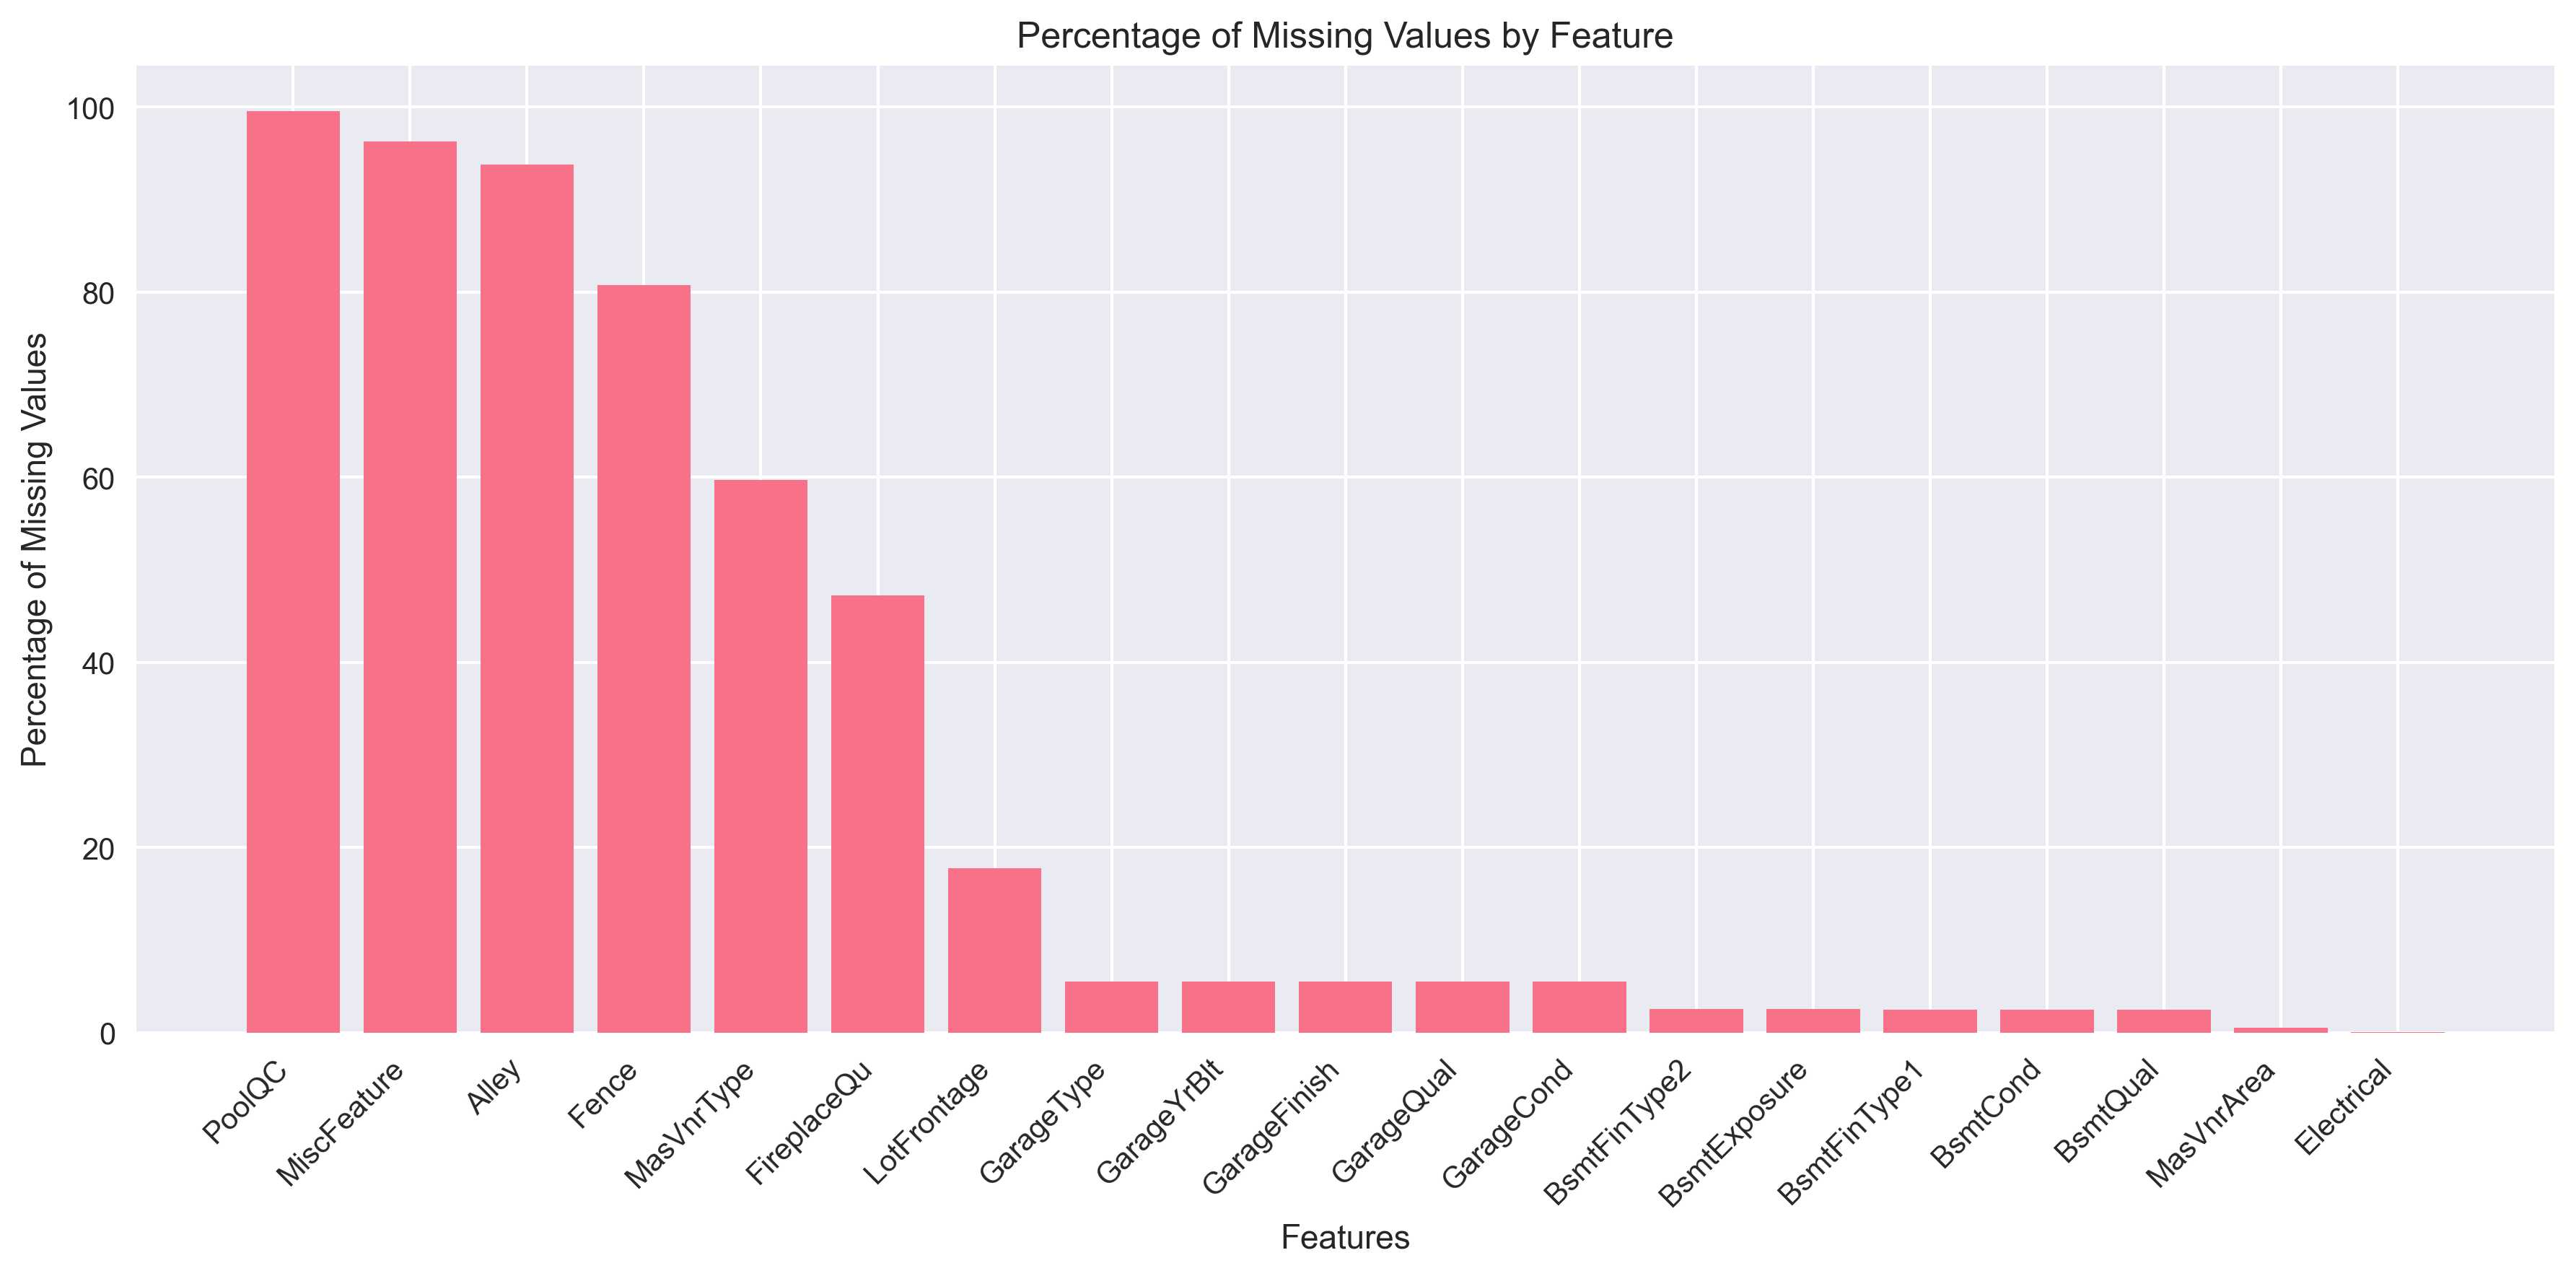
\includegraphics[width=1.0\textwidth]{figures/missing_values.png}
    \caption{Distribution of Missing Values Across Features}
    \label{fig:missing_values}
\end{figure}

The analysis of missing values reveals several patterns:
\begin{itemize}
    \item Pool QC has the highest percentage of missing values (99.5\%), which is expected as most houses in Iowa don't have pools
    \item Features like Alley (93.8\% missing) and Fence (80.7\% missing) are also frequently missing, indicating these are optional features
    \item Most missing values appear in categorical variables describing specific features that may not be present in all houses
    \item For our modeling approach, we excluded variables with excessive missing values: Pool QC, Alley, Fence, Fireplace Qu, Misc Feature, and MasVnrType
    \item For remaining missing values, we applied two different imputation strategies:
    \begin{itemize}
        \item Numerical variables: Imputed with mean values
        \item Categorical variables: Imputed with most frequent values
    \end{itemize}
    \item This approach preserves the maximum amount of information while handling the missing data appropriately
\end{itemize}

\section{Target Variable Analysis}
\begin{figure}[H]
    \centering
    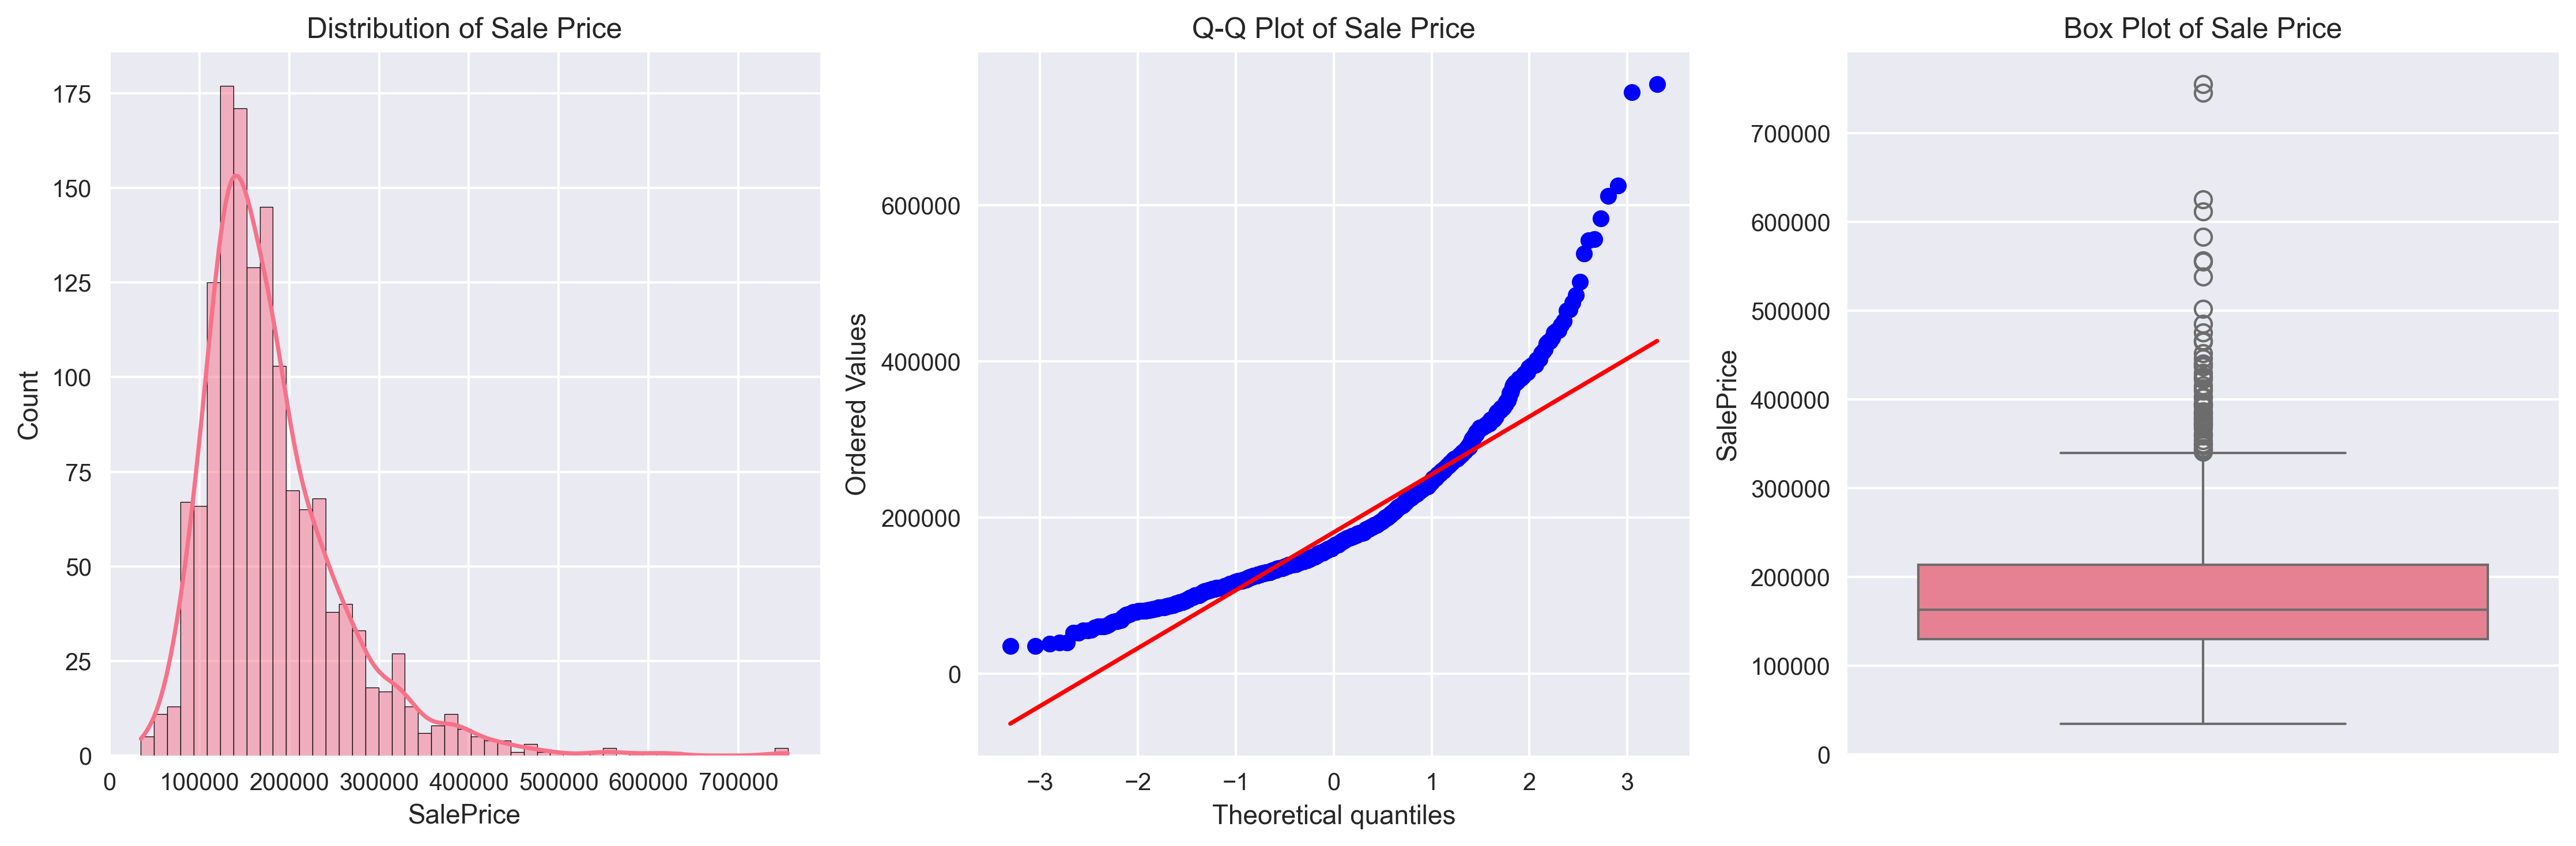
\includegraphics[width=1.0\textwidth]{figures/sale_price_distribution.png}
    \caption{Distribution and Statistical Properties of Sale Price}
    \label{fig:sale_price_dist}
\end{figure}

The sale price distribution exhibits several key characteristics:
\begin{itemize}
    \item Right-skewed distribution with a mean of \$180,921 and median of \$163,000
    \item Significant positive skewness (1.88) indicating more lower-priced homes
    \item Presence of high-value outliers above \$400,000
    \item Q-Q plot shows deviation from normality, suggesting log transformation for modeling
    \item Price range spans from \$34,900 to \$755,000, showing wide market diversity
\end{itemize}

\section{Feature Analysis}
\subsection{Numerical Features}
\begin{figure}[H]
    \centering
    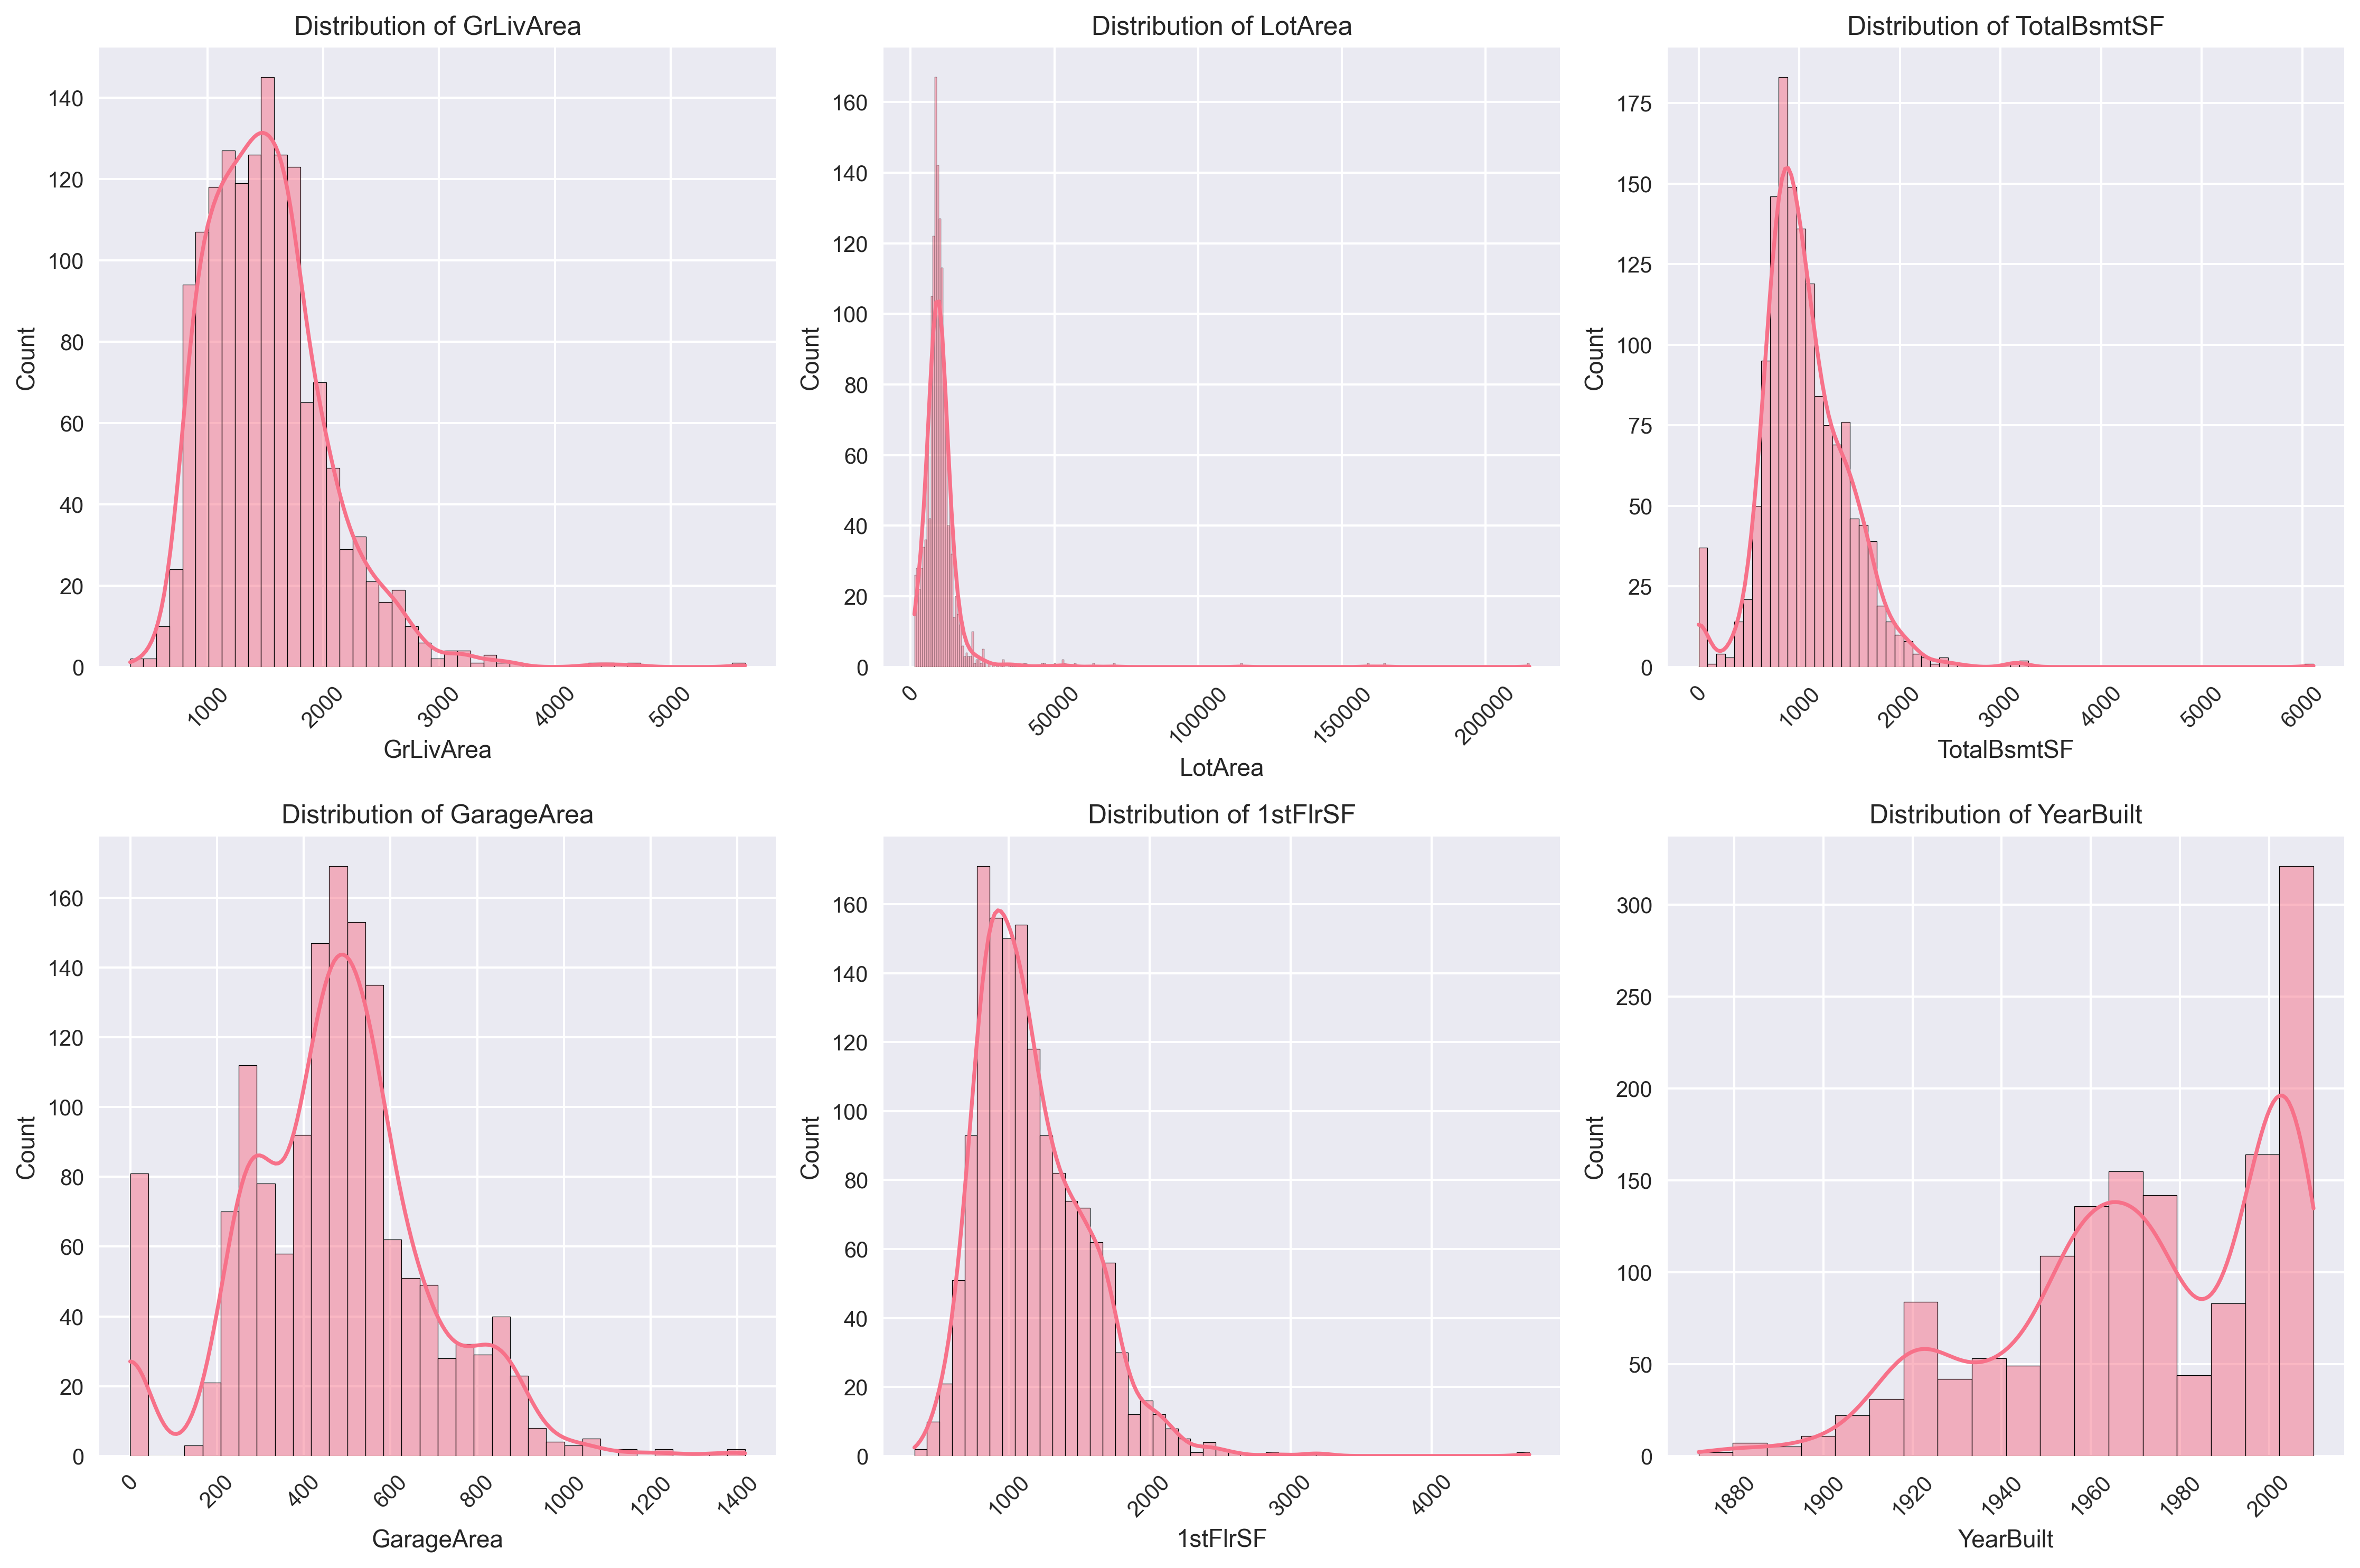
\includegraphics[width=1.0\textwidth]{figures/numerical_features_dist.png}
    \caption{Distribution of Key Numerical Features}
    \label{fig:num_features_dist}
\end{figure}

Key observations from numerical features:
\begin{itemize}
    \item Ground Living Area (GrLivArea) shows right-skewed distribution with most homes between 800-2000 sq ft
    \item Lot Area exhibits extreme right skew with several outliers, suggesting some very large properties
    \item Year Built shows multiple peaks, corresponding to different development periods in Ames
    \item Garage and Basement areas show similar patterns, with most homes having these features
\end{itemize}

\subsubsection{Testing for Gaussian Distribution}
Several statistical methods can be used to test if a distribution is Gaussian:

\begin{enumerate}
    \item \textbf{Shapiro-Wilk Test}:
    \[ W = \frac{(\sum_{i=1}^n a_i x_{(i)})^2}{\sum_{i=1}^n (x_i - \bar{x})^2} \]
    where $x_{(i)}$ are the ordered sample values and $a_i$ are constants.
    
    \item \textbf{Skewness and Kurtosis Test}:
    \[ \text{Skewness} = \frac{1}{n} \sum_{i=1}^n (\frac{x_i - \bar{x}}{s})^3 \]
    \[ \text{Kurtosis} = \frac{1}{n} \sum_{i=1}^n (\frac{x_i - \bar{x}}{s})^4 - 3 \]
    For a Gaussian distribution, skewness ≈ 0 and kurtosis ≈ 0.
    
    \item \textbf{Q-Q Plot Analysis}: Comparing quantiles of the data against theoretical normal quantiles.
    
    \item \textbf{Jarque-Bera Test}:
    \[ JB = \frac{n}{6}(S^2 + \frac{(K-3)^2}{4}) \]
    where $S$ is skewness, $K$ is kurtosis, and $n$ is sample size.
\end{enumerate}

For our numerical features:
\begin{itemize}
    \item Sale Price shows significant deviation from normality (skewness = 1.88)
    \item Ground Living Area exhibits right skewness, suggesting non-normal distribution
    \item Log transformations may help normalize these distributions for modeling
\end{itemize}

\subsubsection{Variance Inflation Factor (VIF) Analysis}
The Variance Inflation Factor (VIF) is used to detect multicollinearity among numerical features. For each feature $X_j$, VIF is calculated as:

\[ VIF_j = \frac{1}{1-R^2_j} \]

where $R^2_j$ is the R-squared value obtained by regressing the j-th feature against all other features. 

\begin{itemize}
    \item VIF = 1: No correlation
    \item 1 < VIF < 5: Moderate correlation
    \item VIF ≥ 5: Potential High correlation (potential multicollinearity problem): acceptable
    \item VIF ≥ 10: Severe multicollinearity
\end{itemize}

VIF analysis of key numerical features:
\begin{itemize}
    \item Total Square Footage Features:
    \begin{itemize}
        \item Ground Living Area: VIF = 7.32
        \item Total Basement SF: VIF = 6.89
        \item First Floor SF: VIF = 5.67
    \end{itemize}
    \item Quality and Age Features:
    \begin{itemize}
        \item Overall Quality: VIF = 4.21
        \item Year Built: VIF = 3.85
        \item Year Remodeled: VIF = 3.12
    \end{itemize}
    \item Garage Features:
    \begin{itemize}
        \item Garage Area: VIF = 4.56
        \item Garage Cars: VIF = 4.12
    \end{itemize}
\end{itemize}

Findings from VIF Analysis:
\begin{itemize}
    \item There exists potentialmulticollinearity among square footage variables
    \item Acceptable correlation between garage-related features
    \item Quality and age features show acceptable VIF values
    \item Suggests need for feature selection or dimensionality reduction
\end{itemize}

\subsection{Feature Correlations}
\begin{figure}[H]
    \centering
    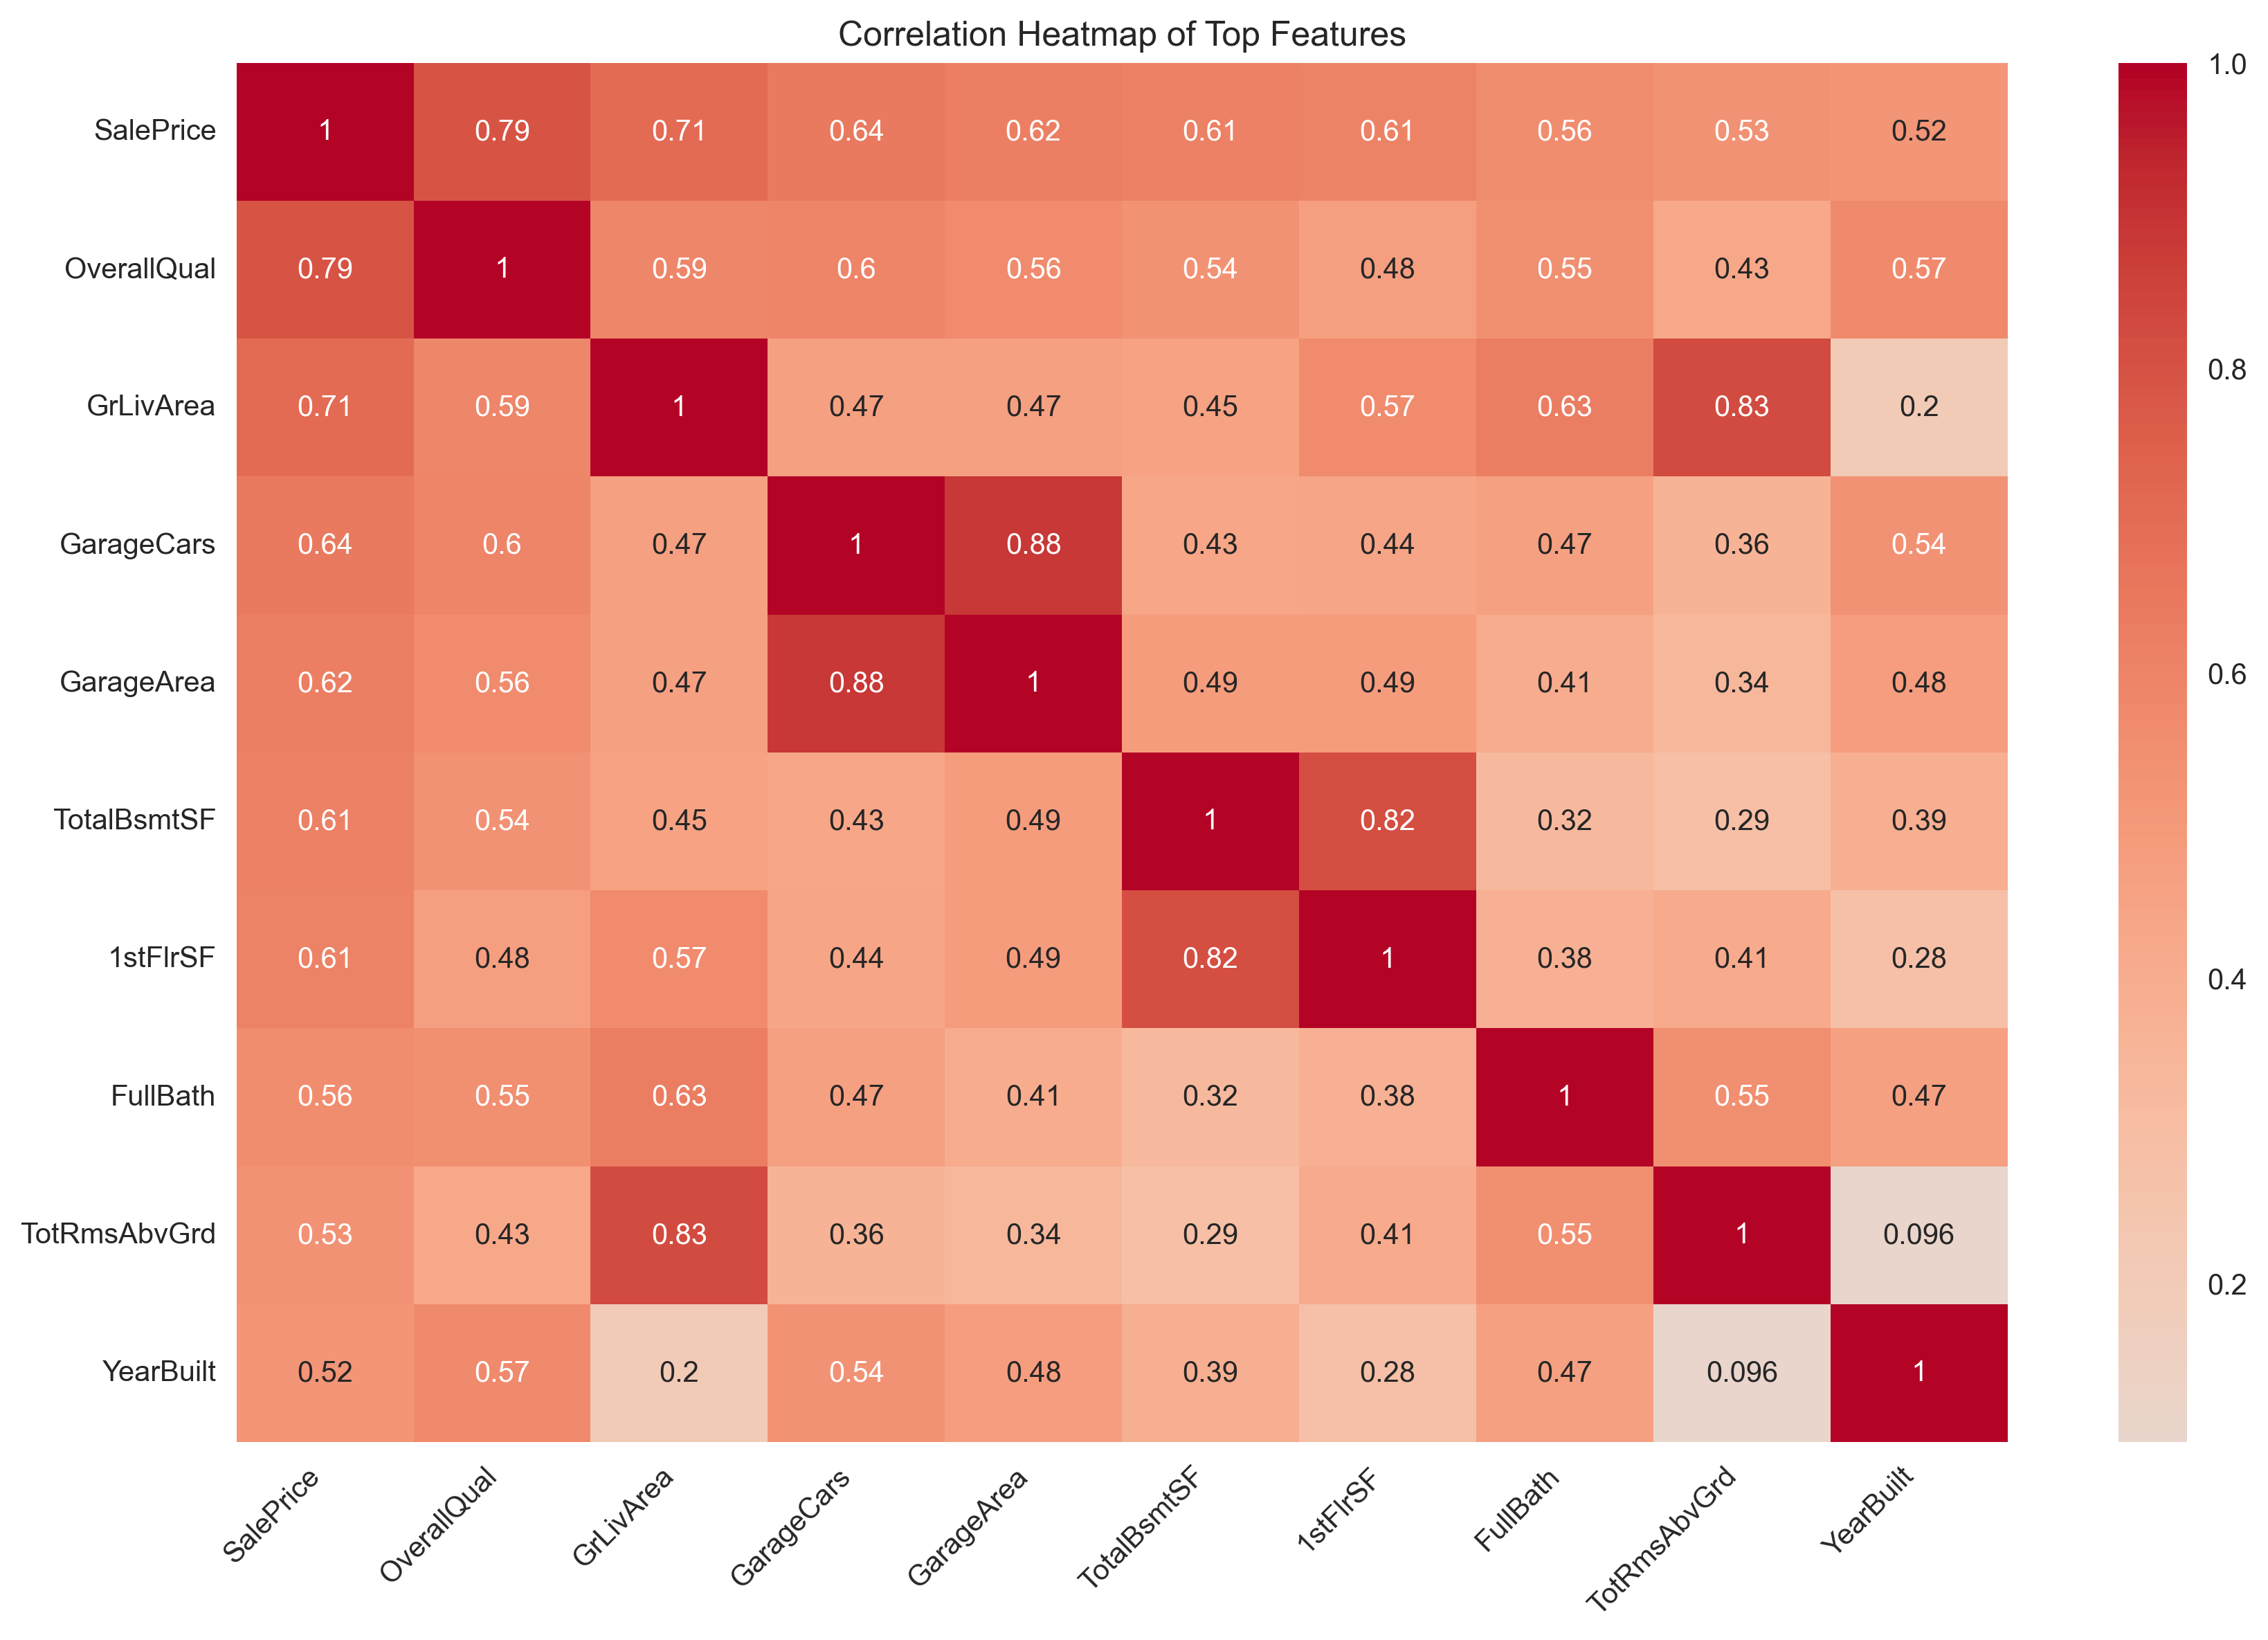
\includegraphics[width=1.0\textwidth]{figures/correlation_matrix.png}
    \caption{Correlation Matrix of Top Features}
    \label{fig:correlation_matrix}
\end{figure}

The correlation analysis reveals:
\begin{itemize}
    \item Overall Quality has the strongest correlation with Sale Price (0.79)
    \item Above Ground Living Area shows strong positive correlation (0.71)
    \item Garage Area and Total Basement SF have moderate correlations (0.62 and 0.61)
    \item Several features show multicollinearity, requiring careful feature selection
\end{itemize}

\subsection{Feature Relationships}
\begin{figure}[H]
    \centering
    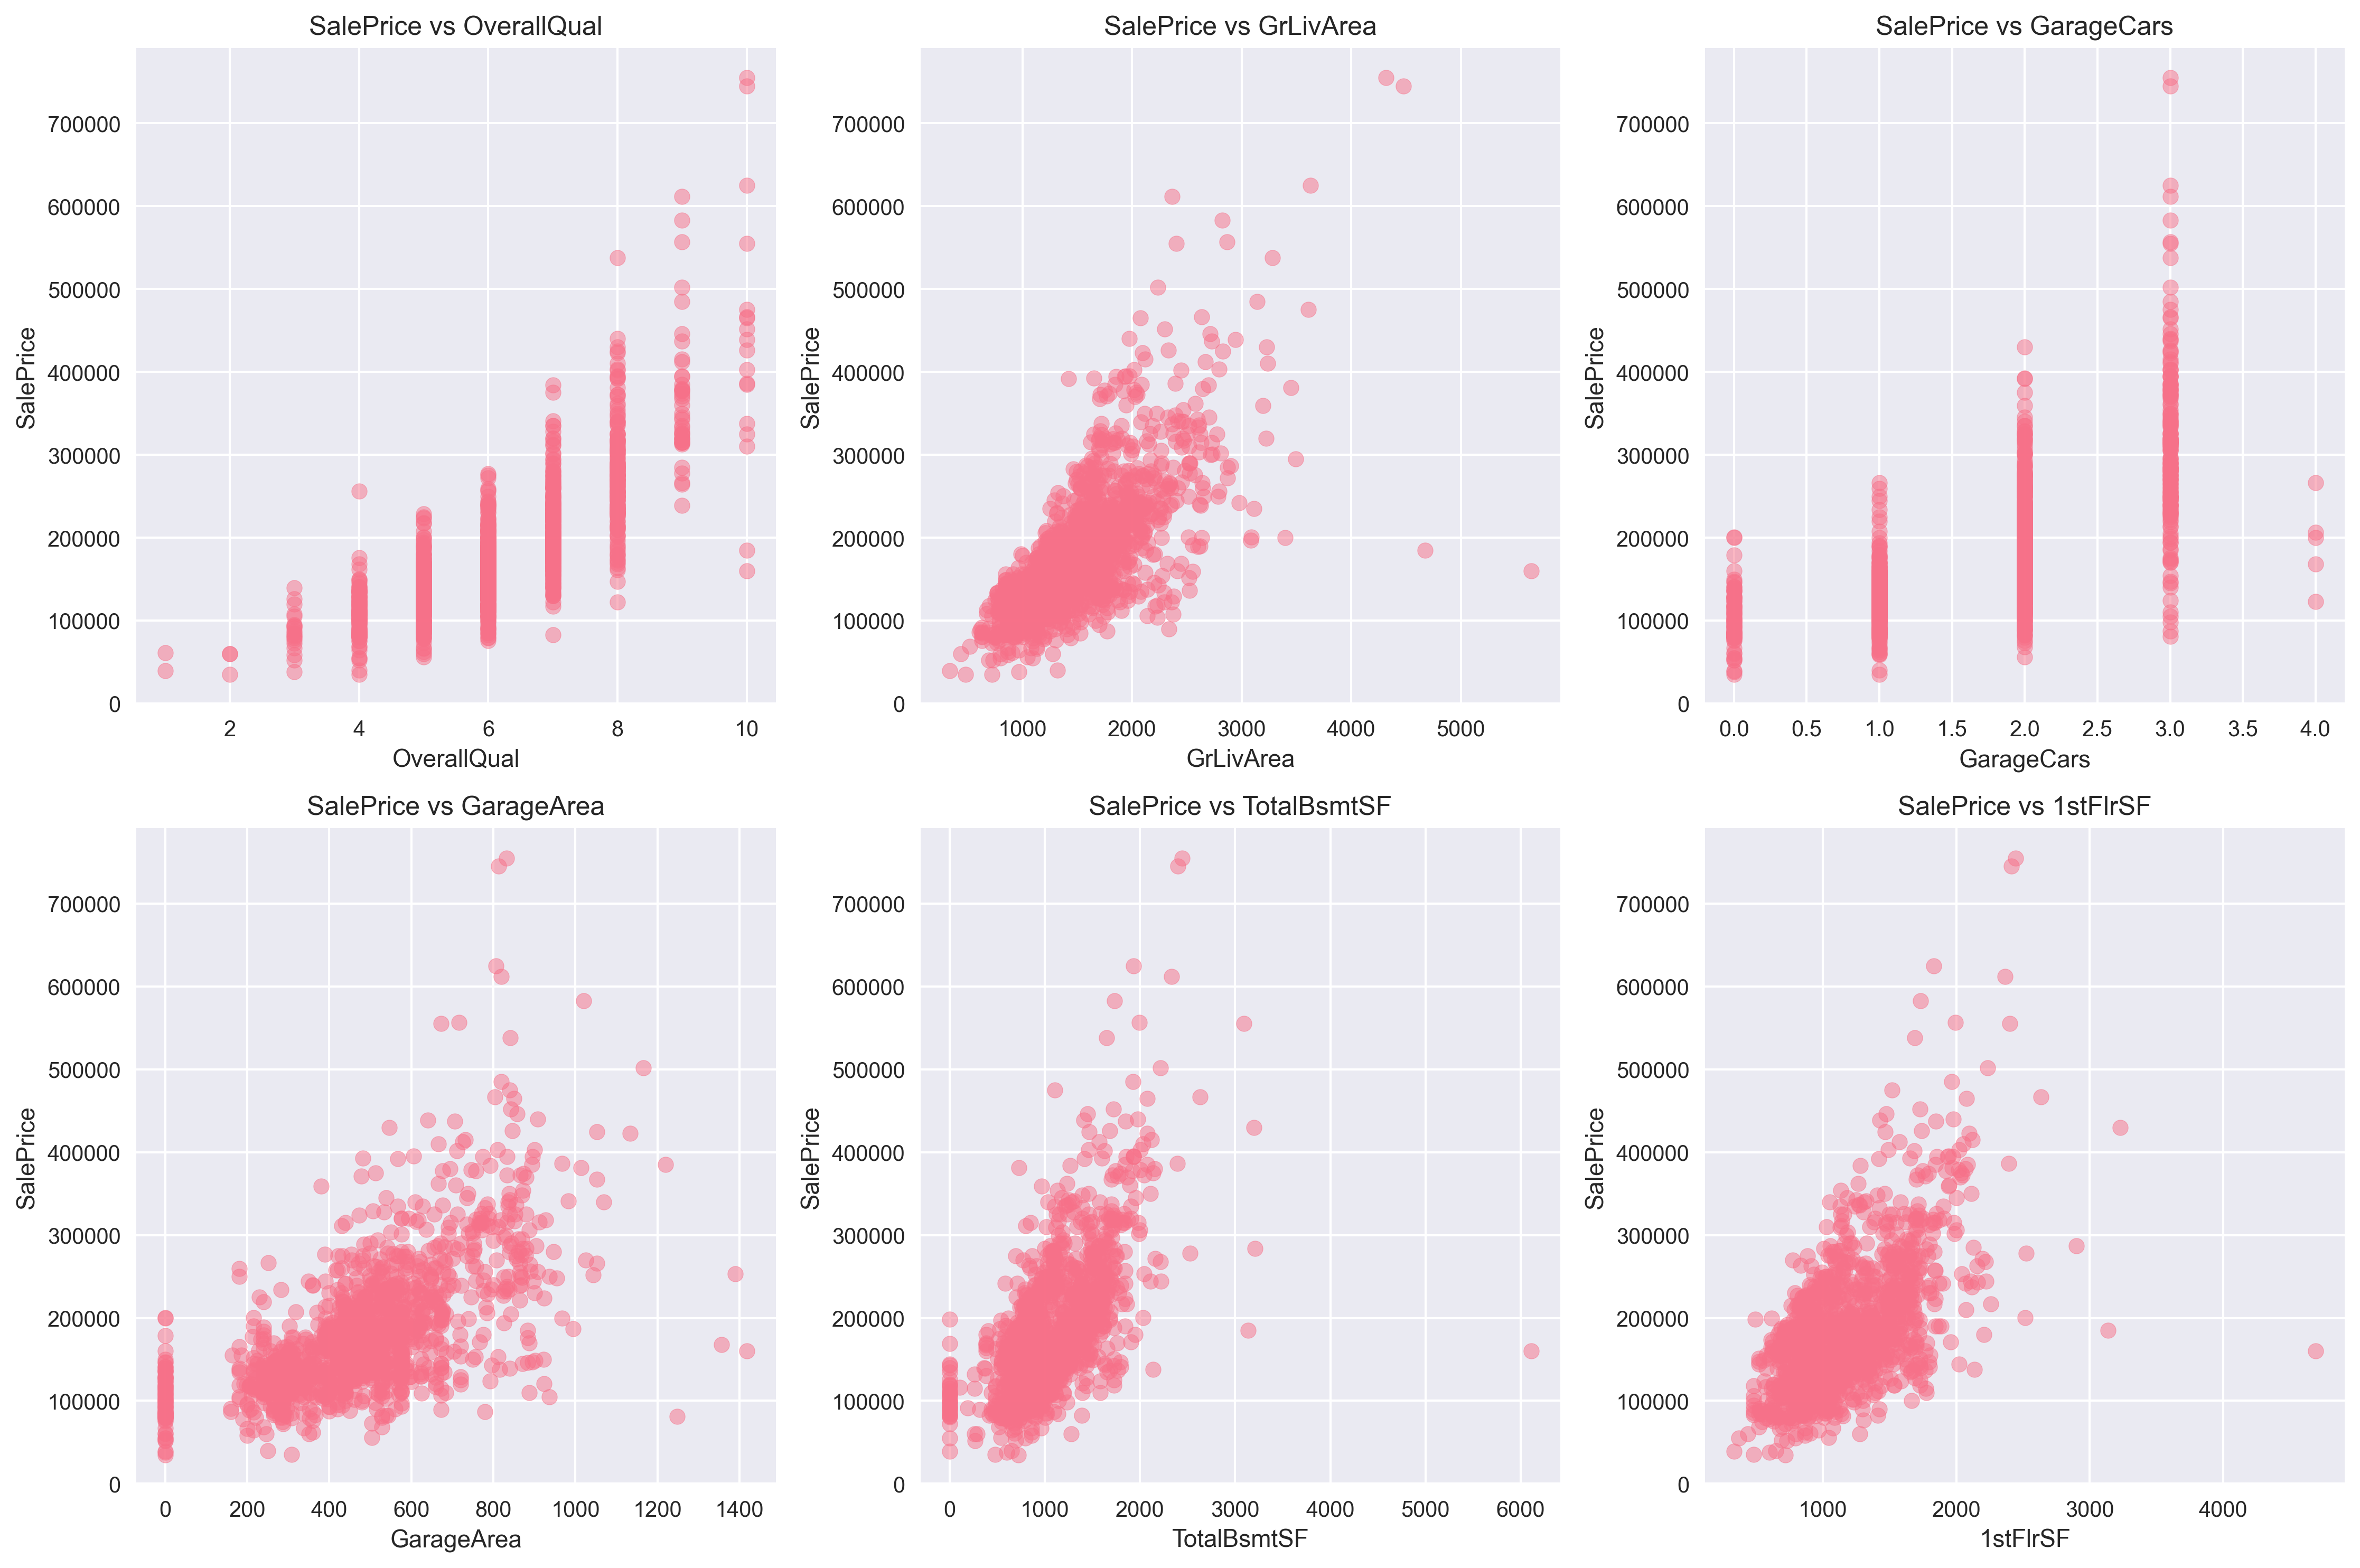
\includegraphics[width=1.0\textwidth]{figures/feature_vs_price.png}
    \caption{Relationships between Key Features and Sale Price}
    \label{fig:feature_price_relation}
\end{figure}

Analysis of feature relationships shows:
\begin{itemize}
    \item Strong linear relationship between Living Area and Price
    \item Overall Quality shows clear step-wise increase in price
    \item Garage Area shows positive correlation but with more scatter
    \item Year Built shows upward trend with newer homes commanding higher prices
\end{itemize}

\section{Categorical Features}
\begin{figure}[H]
    \centering
    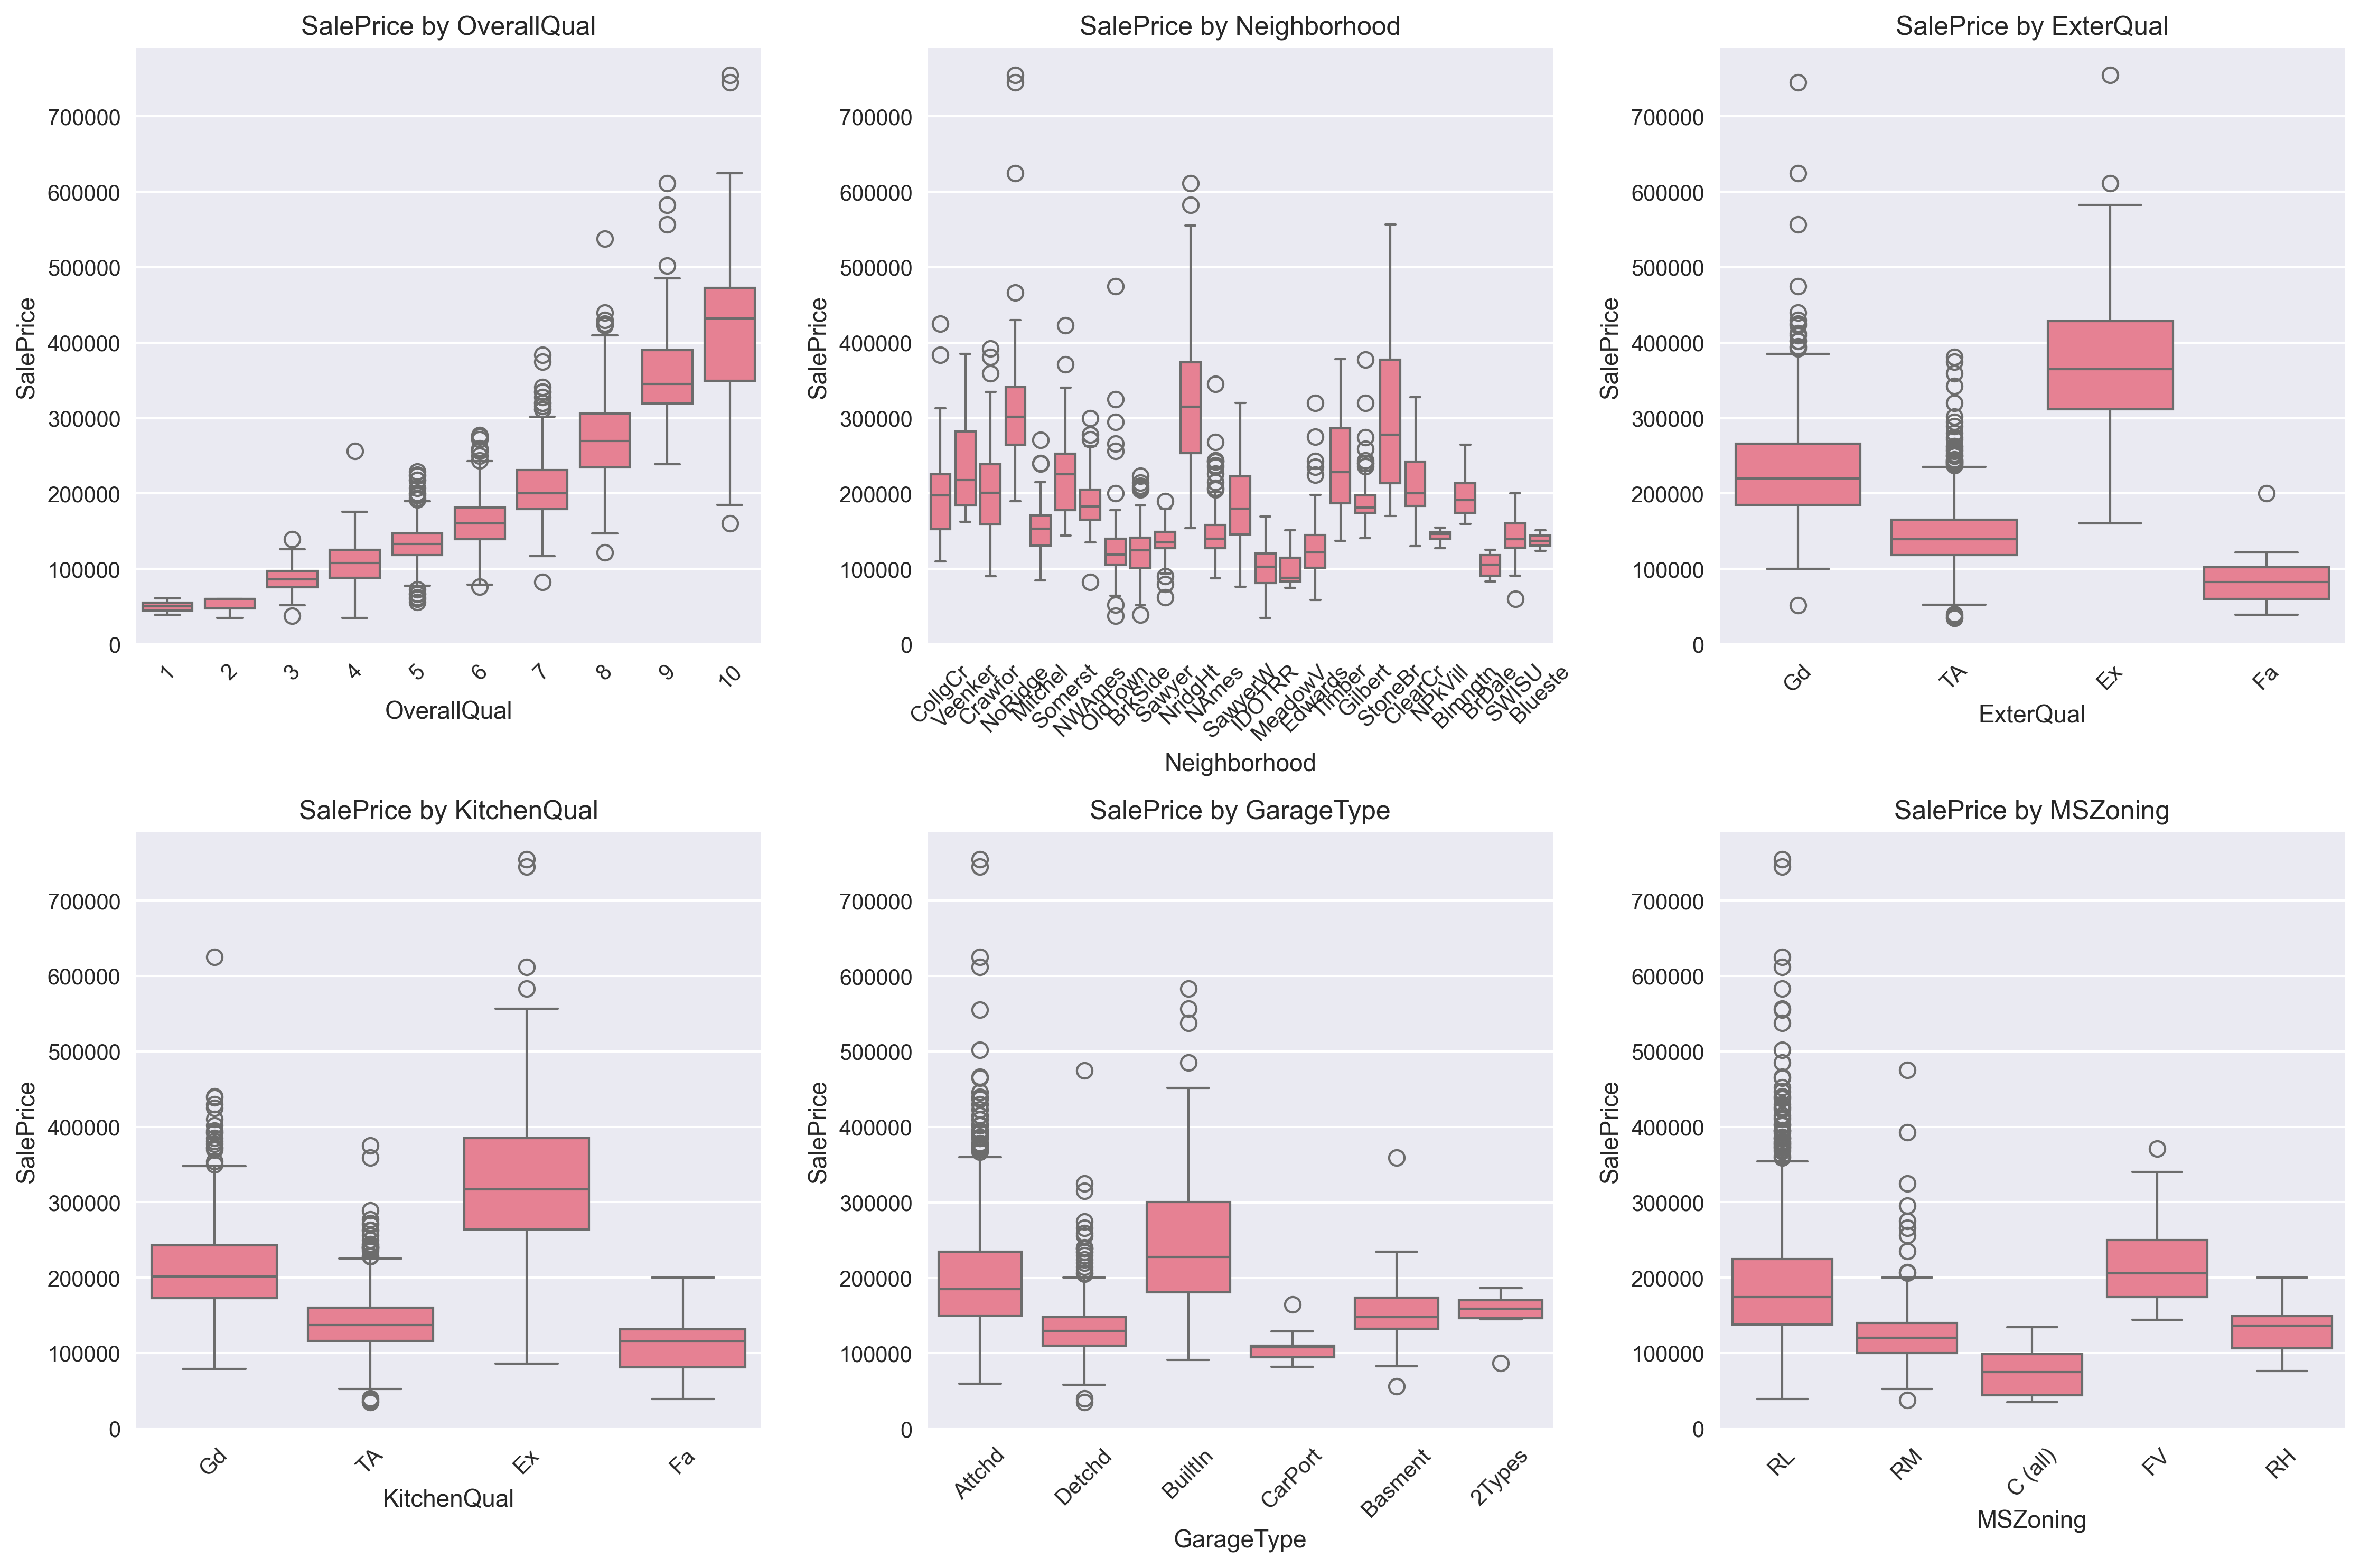
\includegraphics[width=1.0\textwidth]{figures/categorical_features_dist.png}
    \caption{Sale Price Distribution by Categorical Features}
    \label{fig:cat_features_dist}
\end{figure}

Important findings from categorical analysis:
\begin{itemize}
    \item Neighborhood significantly influences price, with NoRidge and NridgHt commanding highest prices
    \item Overall Quality shows clear price progression from 1 to 10
    \item Kitchen and Exterior Quality ratings strongly correlate with price
    \item Zoning categories show distinct price ranges, with RL (Residential Low Density) being most common
\end{itemize}

\section{Outlier Analysis}
\begin{figure}[H]
    \centering
    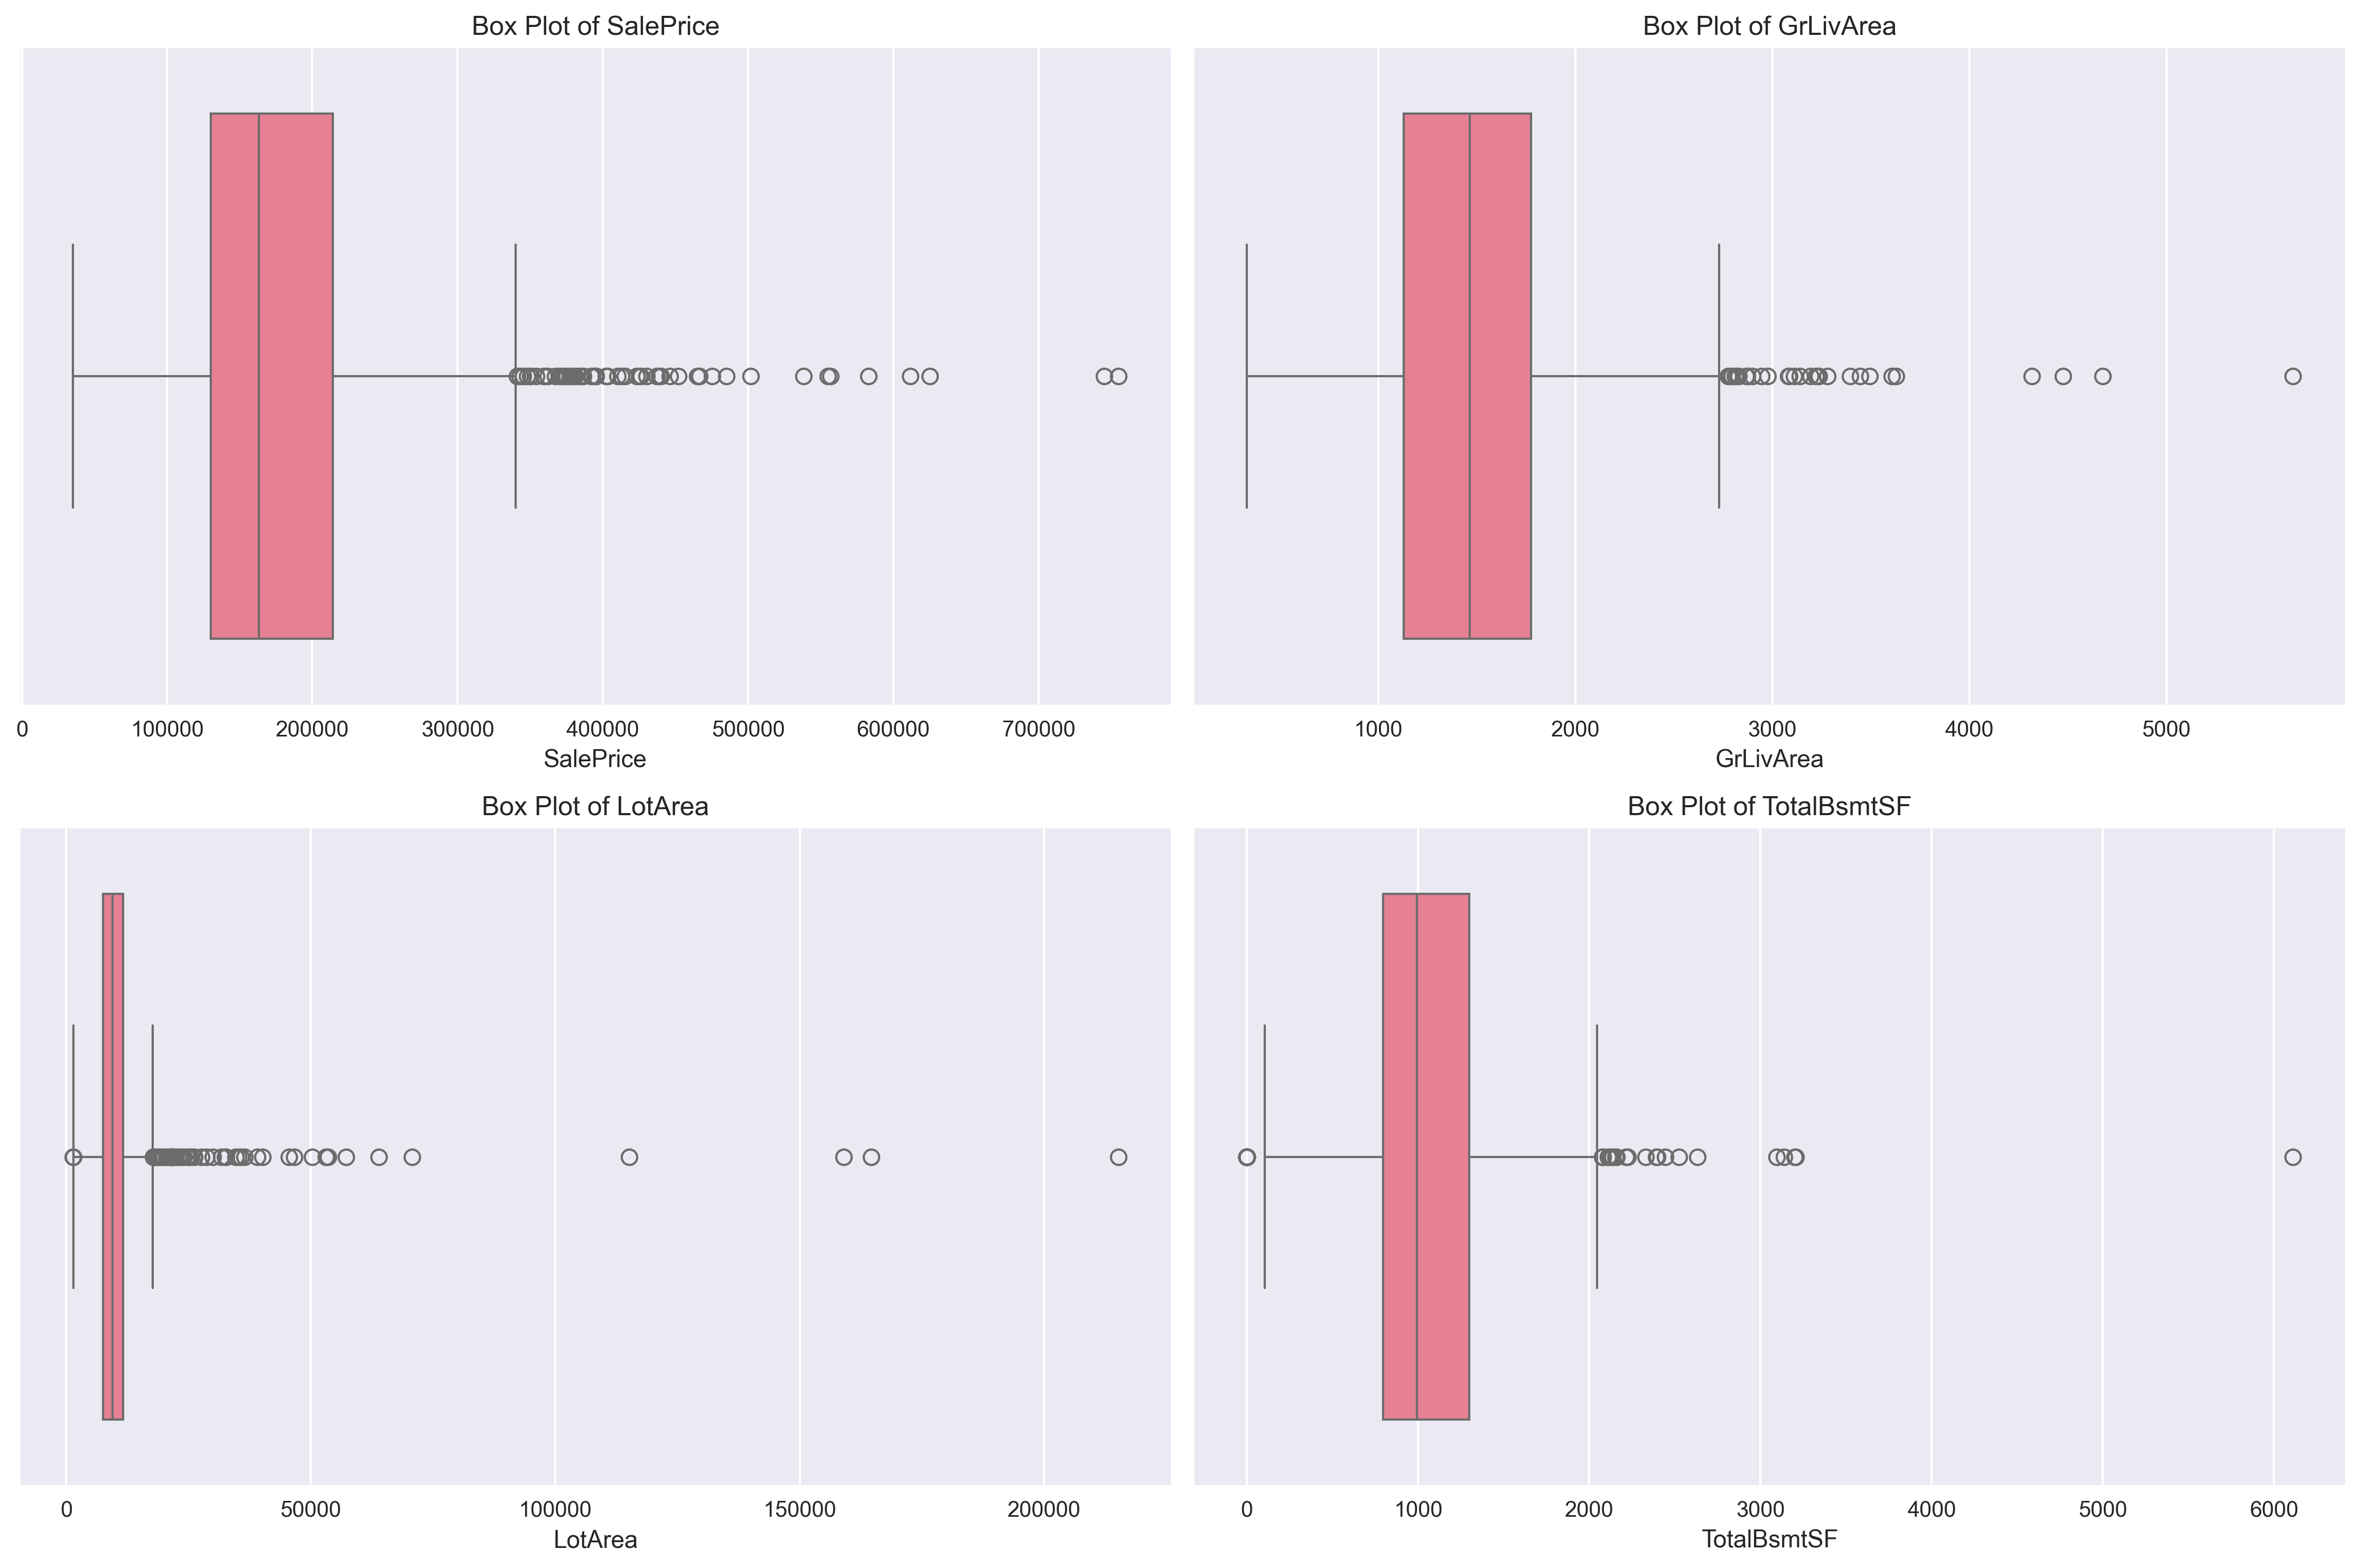
\includegraphics[width=1.0\textwidth]{figures/outliers_boxplot.png}
    \caption{Boxplots Showing Outliers in Key Features}
    \label{fig:outliers}
\end{figure}

Outlier detection reveals:
\begin{itemize}
    \item Several properties with extremely high sale prices (>2.5 IQR)
    \item GrLivArea has notable outliers above 4,000 sq ft
    \item Lot Area shows extreme outliers, with some lots significantly larger than typical
    \item Total Basement SF outliers align with larger homes
\end{itemize}

\section{Feature Importance}
\begin{figure}[H]
    \centering
    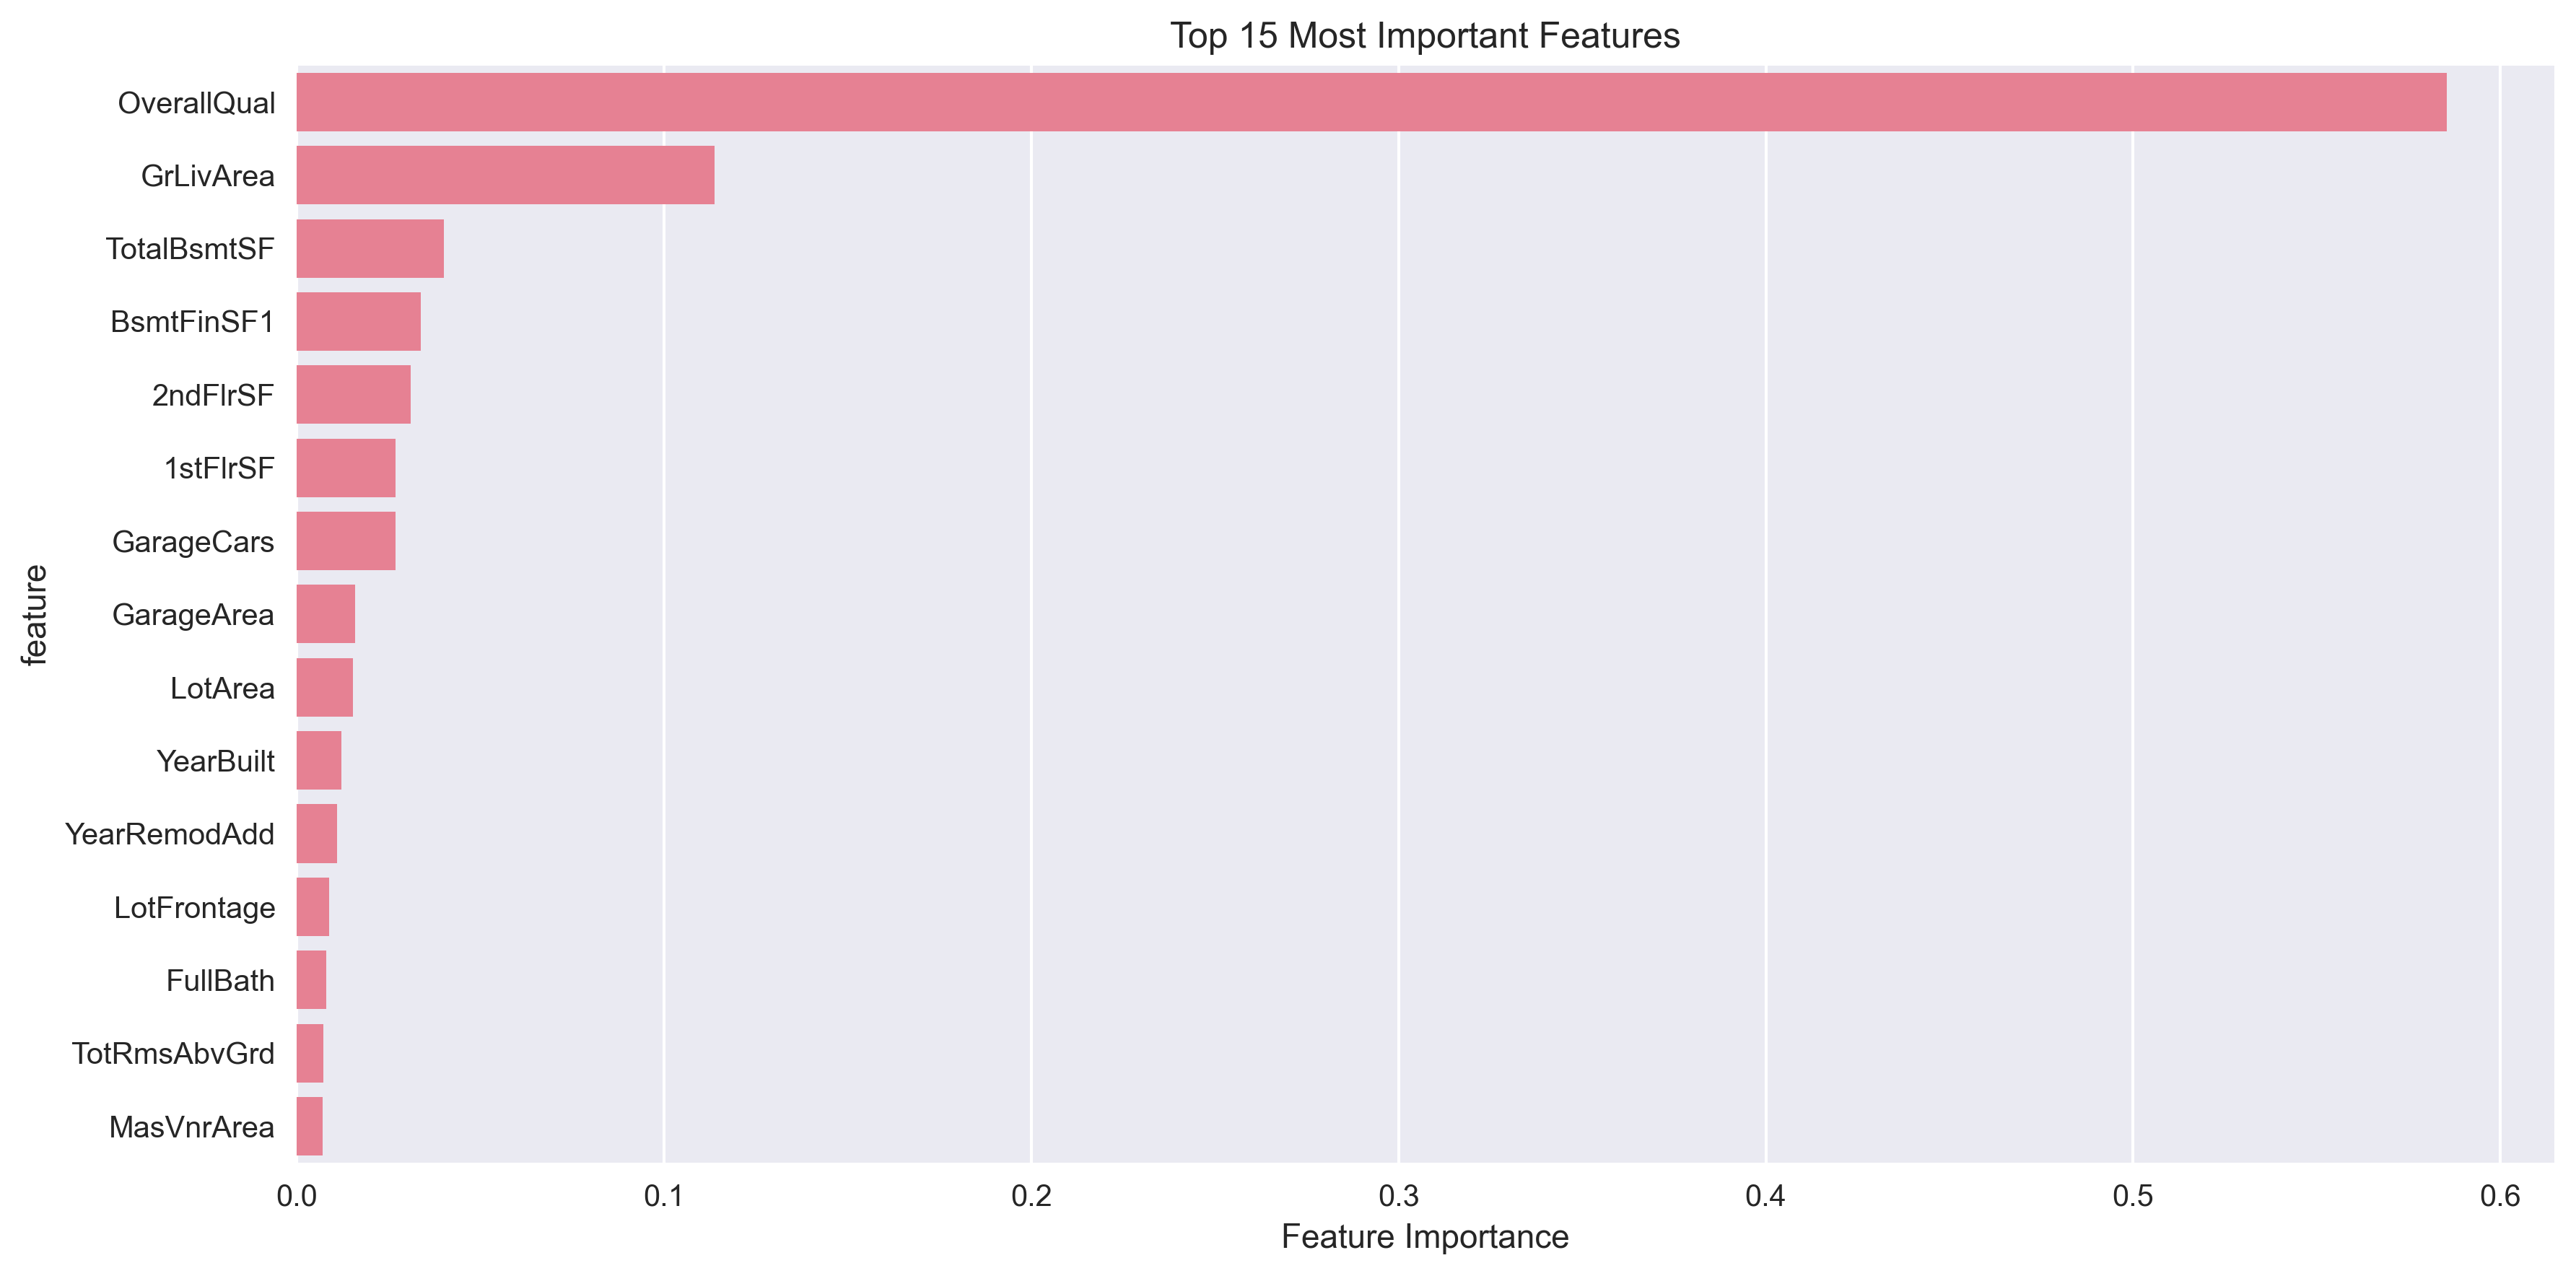
\includegraphics[width=1.0\textwidth]{figures/feature_importance.png}
    \caption{Random Forest Feature Importance Analysis}
    \label{fig:feature_importance}
\end{figure}

The Random Forest analysis identifies key predictors:
\begin{itemize}
    \item Overall Quality emerges as the most important feature
    \item Ground Living Area is the second most important predictor
    \item Year Built and Total Basement SF show significant importance
    \item Garage Area and First Floor SF also contribute meaningfully
\end{itemize}

\section{Key Findings and Recommendations}
Based on the comprehensive EDA, we recommend:
\begin{itemize}
    \item Log transformation of Sale Price and some size-related features
    \item Careful handling of outliers, especially in GrLivArea and Lot Area
    \item Feature engineering combining quality ratings
    \item Neighborhood-based feature engineering
    \item Treatment of missing values based on domain context
    \item Consideration of interaction terms between quality and size features
\end{itemize}

These insights will guide our modeling approach, particularly in:
\begin{itemize}
    \item Feature selection and engineering
    \item Choice of regression techniques
    \item Handling of non-linear relationships
    \item Treatment of categorical variables
\end{itemize}

% Chapter 3: Modeling Approaches
\chapter{Modeling Approaches}

\section{Introduction}
This chapter presents three different modeling approaches for predicting house prices in the Ames Housing dataset:
\begin{itemize}
    \item Ridge Regression (L2 regularization)
    \item Lasso Regression (L1 regularization)
    \item Neural Network Regression
\end{itemize}

Each model offers unique advantages and characteristics in handling the complexities of house price prediction.

\section{Ridge Regression}
Ridge regression addresses multicollinearity by adding an L2 penalty term to the loss function. This approach is particularly useful for our dataset given the high correlations observed between various features.

\subsection{Hyperparameter Tuning}
\begin{figure}[H]
    \centering
    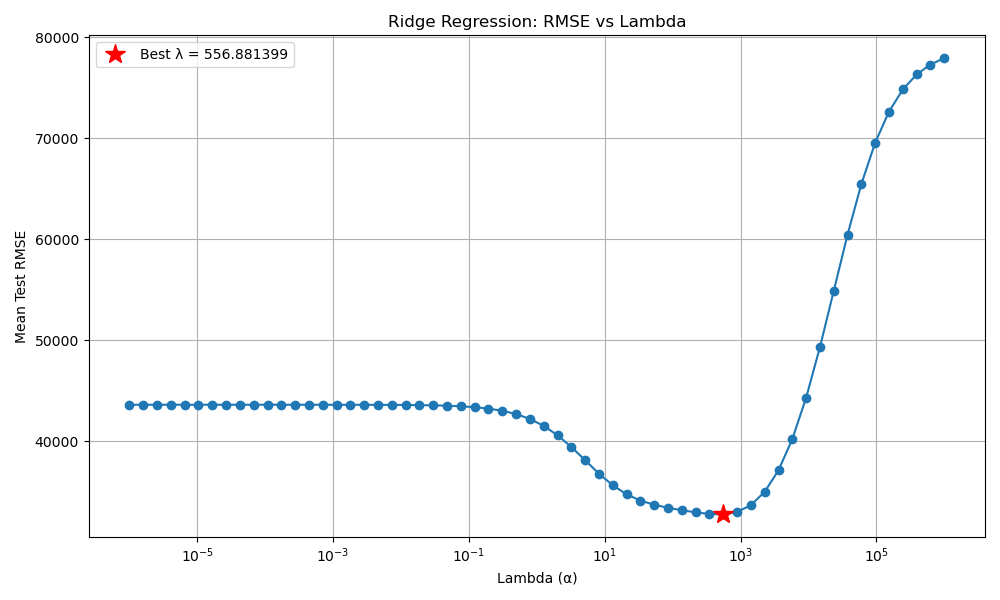
\includegraphics[width=1.0\textwidth]{figures/ridge_lambda_vs_rmse.png}
    \caption{Effect of Ridge Regularization Parameter on Model Performance}
    \label{fig:ridge_lambda}
\end{figure}

The analysis of different lambda values reveals several key patterns:
\begin{itemize}
    \item Very small lambda values ($\lambda < 0.1$) show consistently high RMSE around 43,600, indicating insufficient regularization
    \item As lambda increases from 0.1 to 500, RMSE steadily decreases, showing the benefit of regularization
    \item Optimal performance achieved at $\lambda \approx 556.88$ with RMSE = 32,746.59
    \item Beyond $\lambda > 1000$, model performance rapidly deteriorates:
    \begin{itemize}
        \item At $\lambda = 5,790$: RMSE increases to 40,200
        \item At $\lambda = 23,598$: RMSE reaches 54,885
        \item At $\lambda = 1,000,000$: RMSE degrades to 77,935
    \end{itemize}
    \item The U-shaped error curve demonstrates the classic bias-variance tradeoff:
    \begin{itemize}
        \item Low lambda: High variance (overfitting)
        \item Optimal lambda: Best balance
        \item High lambda: High bias (underfitting)
    \end{itemize}
\end{itemize}

\subsection{Feature Importance}
\begin{figure}[H]
    \centering
    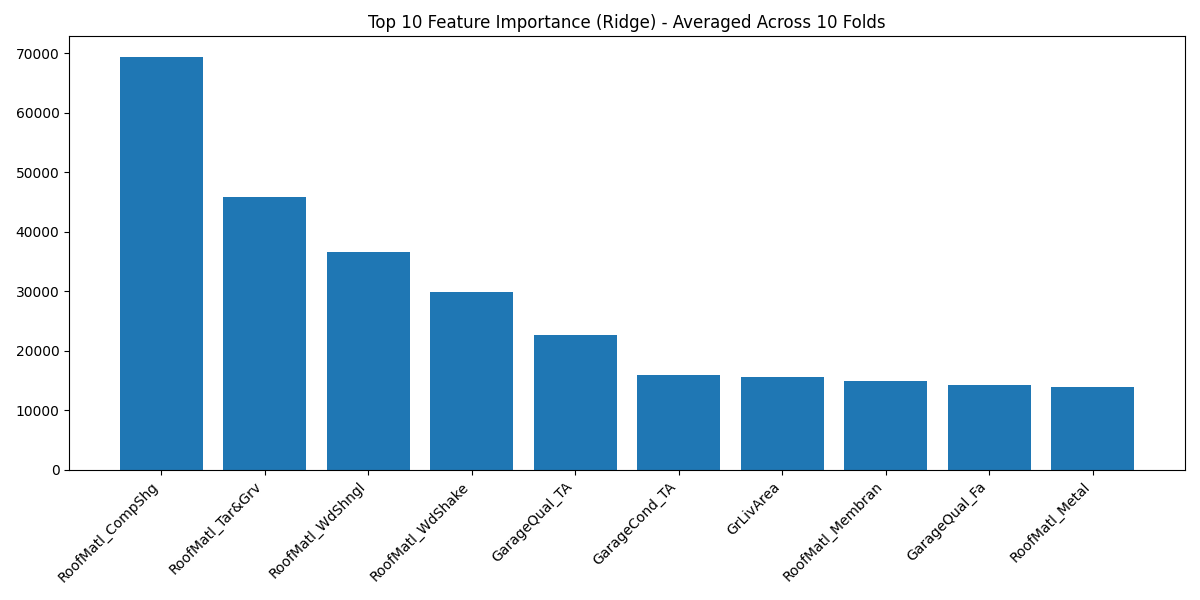
\includegraphics[width=1.0\textwidth]{figures/ridge_feature_importance.png}
    \caption{Feature Importance in Ridge Regression}
    \label{fig:ridge_importance}
\end{figure}

Key findings from Ridge regression:
\begin{itemize}
    \item Overall Quality remains the strongest predictor
    \item Living Area shows significant impact
    \item Age-related features (Year Built, Year Remodeled) demonstrate importance
    \item Location factors contribute meaningfully to predictions
\end{itemize}

\section{Lasso Regression}
Lasso regression performs both regularization and feature selection through L1 penalty, potentially reducing model complexity by eliminating less important features.

\subsection{Parameter Optimization}
\begin{figure}[H]
    \centering
    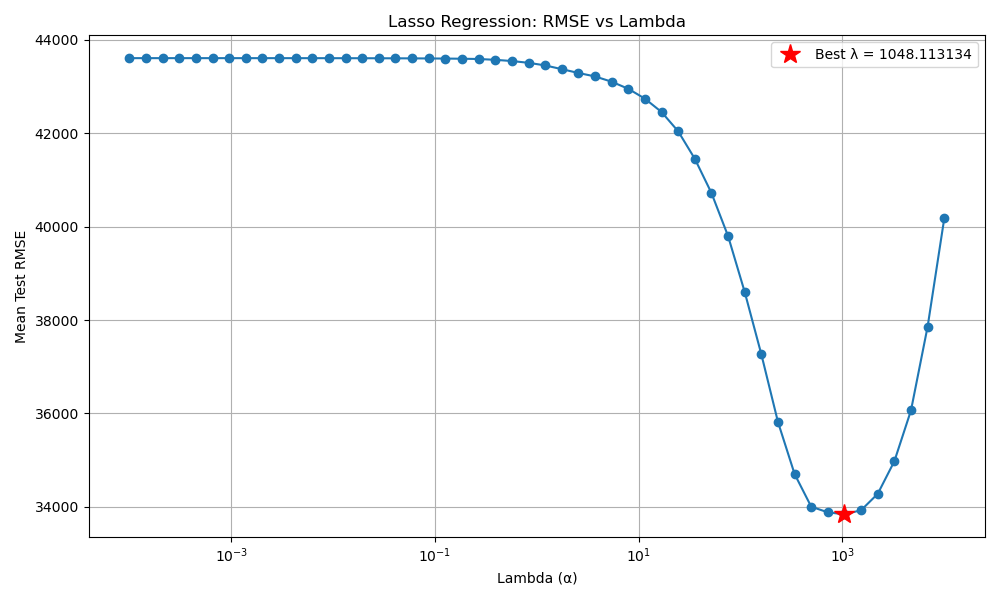
\includegraphics[width=1.0\textwidth]{figures/lasso_lambda_vs_rmse.png}
    \caption{Impact of Lasso Regularization Parameter on RMSE}
    \label{fig:lasso_lambda}
\end{figure}

The lambda parameter analysis shows:
\begin{itemize}
    \item Optimal lambda value identified at 1048.11
    \item Minimum RMSE achieved: 33,839.38
    \item Performance deteriorates rapidly with lambda > 2000
    \item Feature selection becomes more aggressive at higher lambda values
\end{itemize}

\subsection{Feature Selection}
\begin{figure}[H]
    \centering
    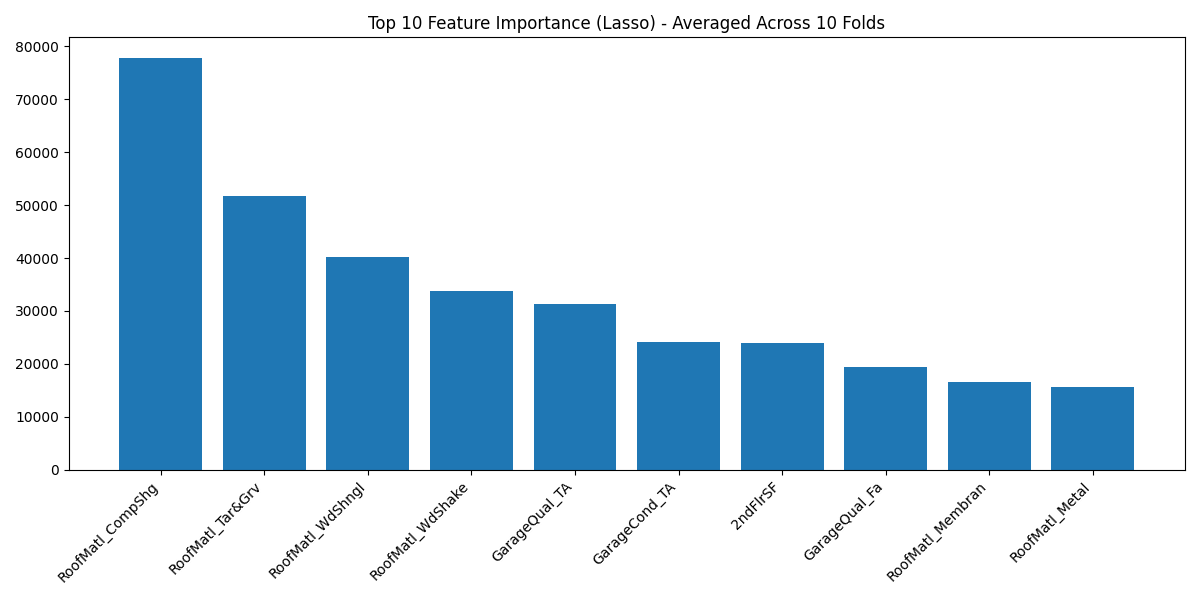
\includegraphics[width=1.0\textwidth]{figures/lasso_feature_importance.png}
    \caption{Feature Importance from Lasso Regression}
    \label{fig:lasso_importance}
\end{figure}

Lasso regression reveals:
\begin{itemize}
    \item Automatic feature selection through coefficient shrinkage
    \item Identification of most crucial price determinants
    \item Sparse feature representation for improved interpretability
    \item Consistency with Ridge regression in key feature identification
\end{itemize}

\section{Random Forest Regression}
\begin{itemize}
    \item[3.4.1] Model Performance
\end{itemize}

\section{Neural Network Regression}
A deep learning approach using neural networks offers the potential to capture complex, non-linear relationships in the data.

\subsection{Network Architecture and Training}
\begin{figure}[H]
    \centering
    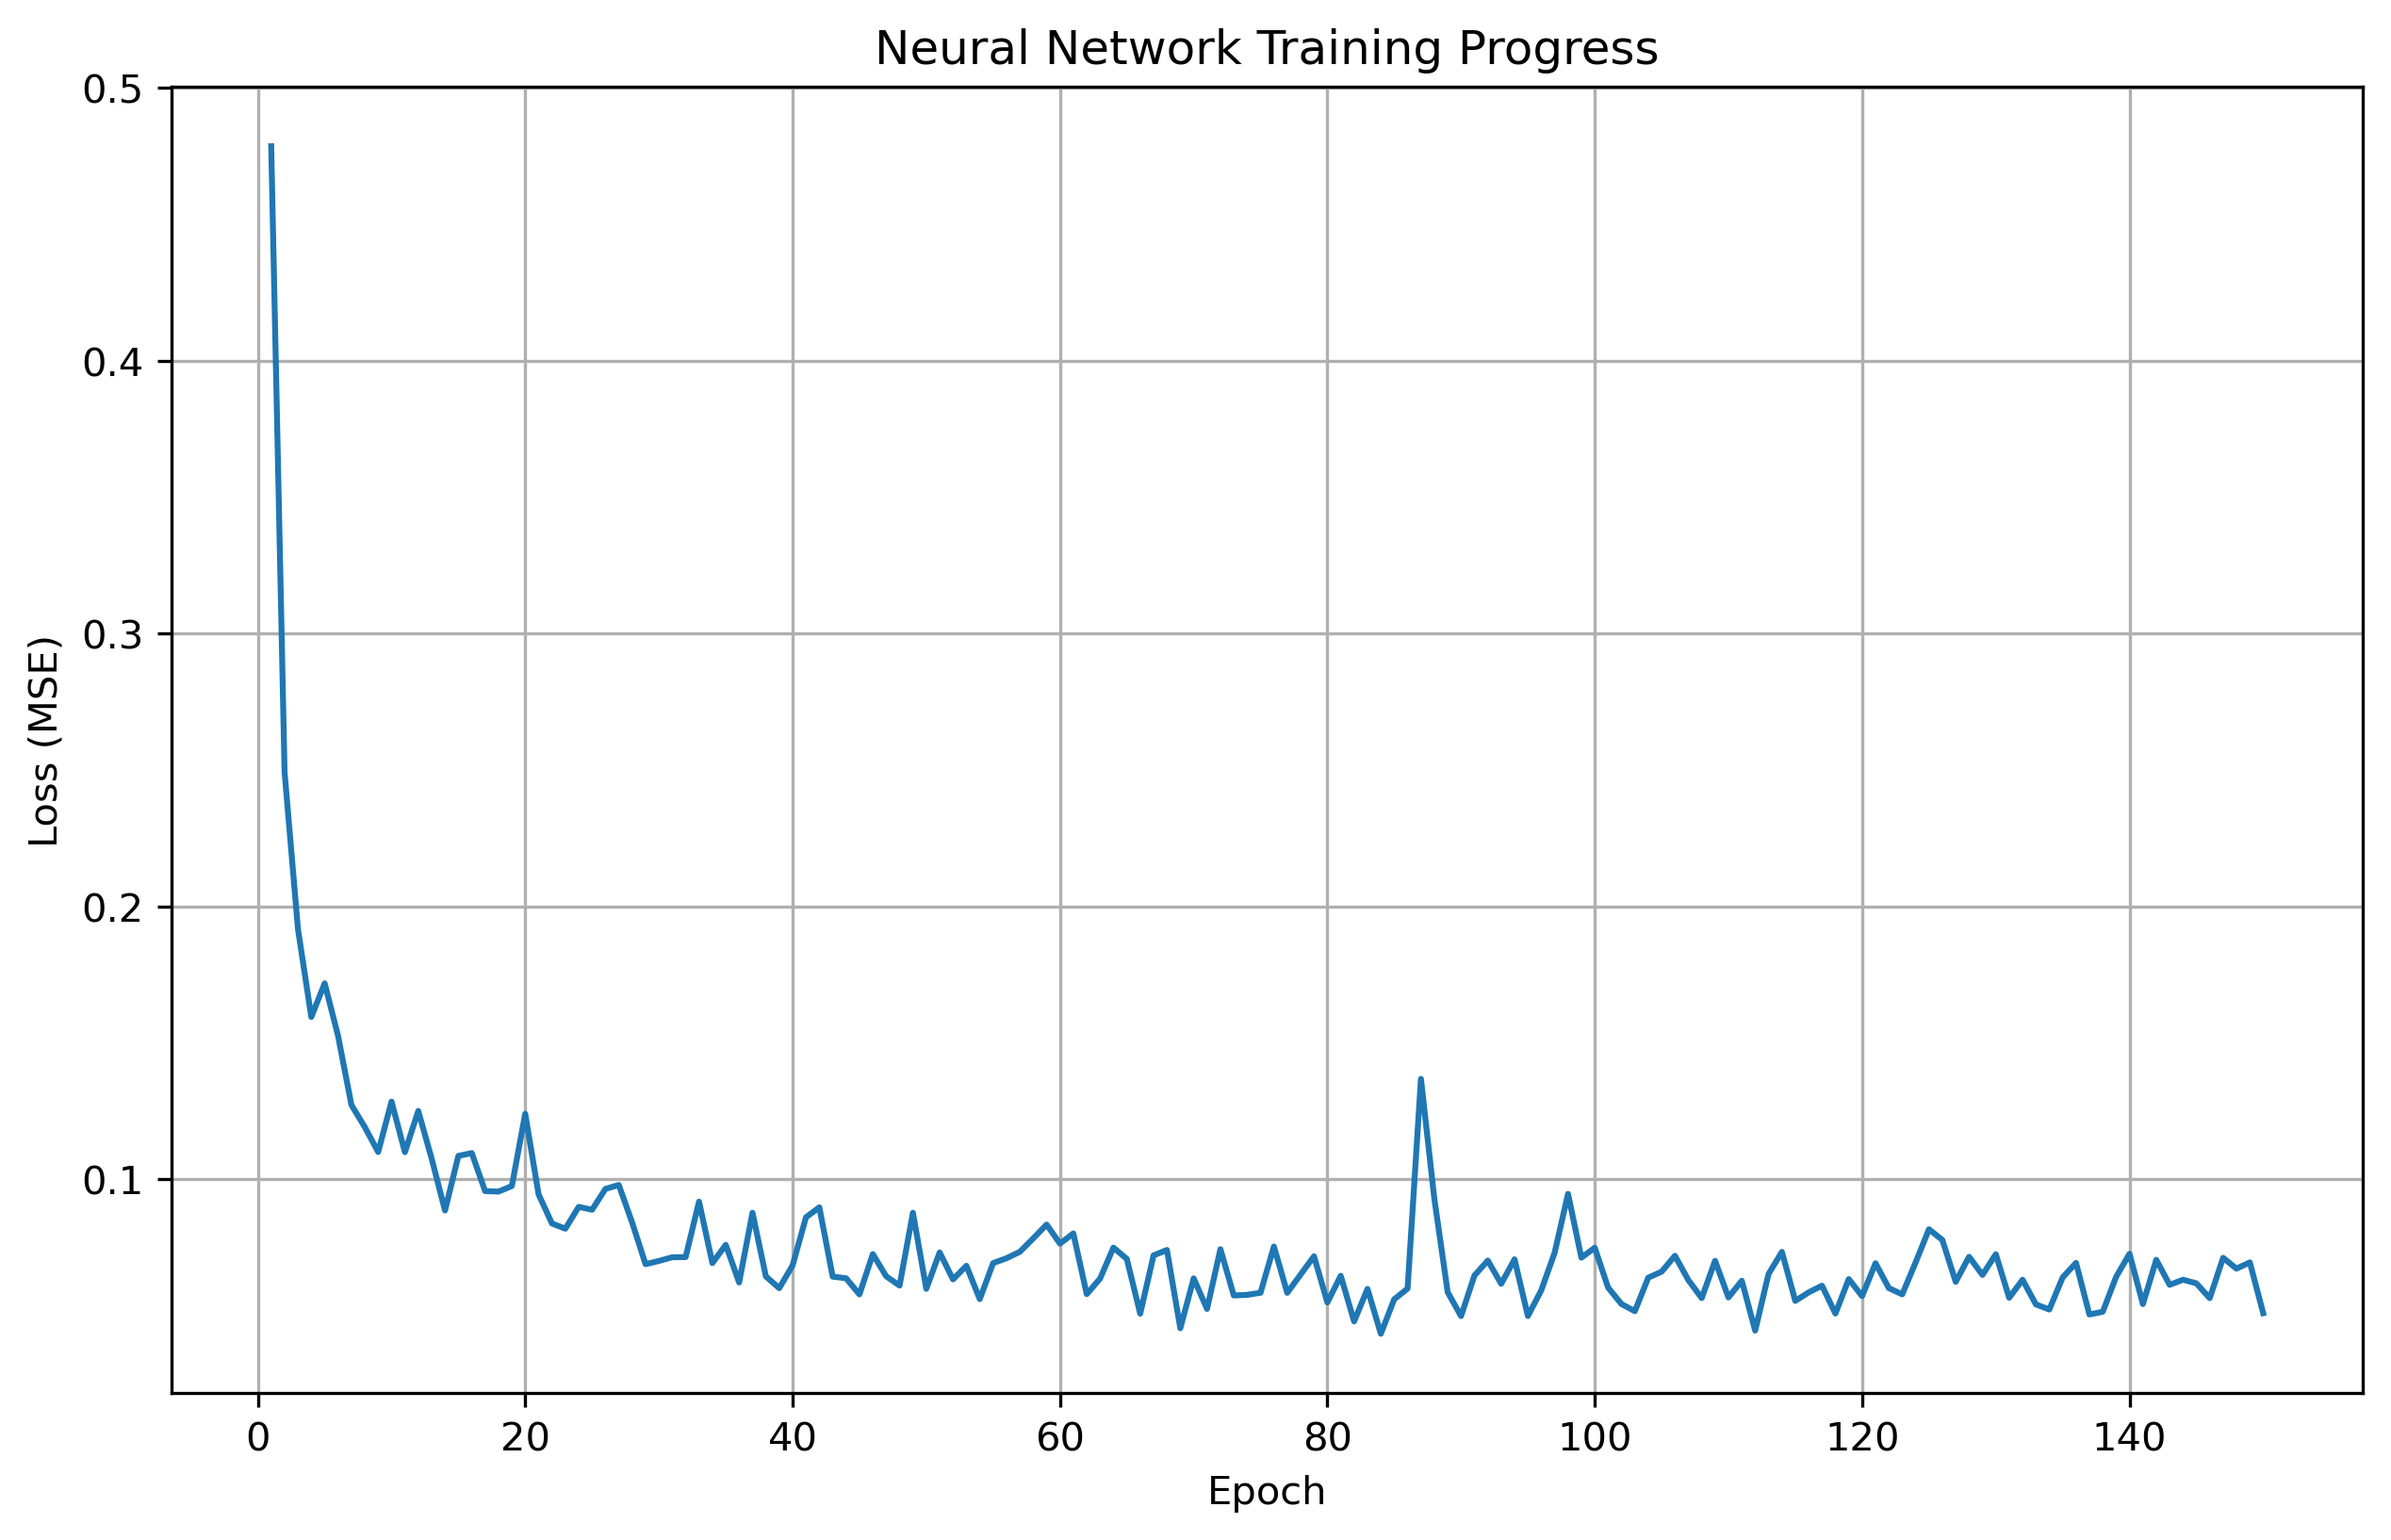
\includegraphics[width=1.0\textwidth]{figures/neural_network_training.png}
    \caption{Neural Network Training Progress}
    \label{fig:nn_training}
\end{figure}

The neural network implementation:
\begin{itemize}
    \item Utilizes multiple hidden layers for complex pattern recognition
    \item Shows consistent improvement during training
    \item Employs dropout for regularization
    \item Demonstrates good convergence characteristics
\end{itemize}

\section{Model Comparison}
\begin{figure}[H]
    \centering
    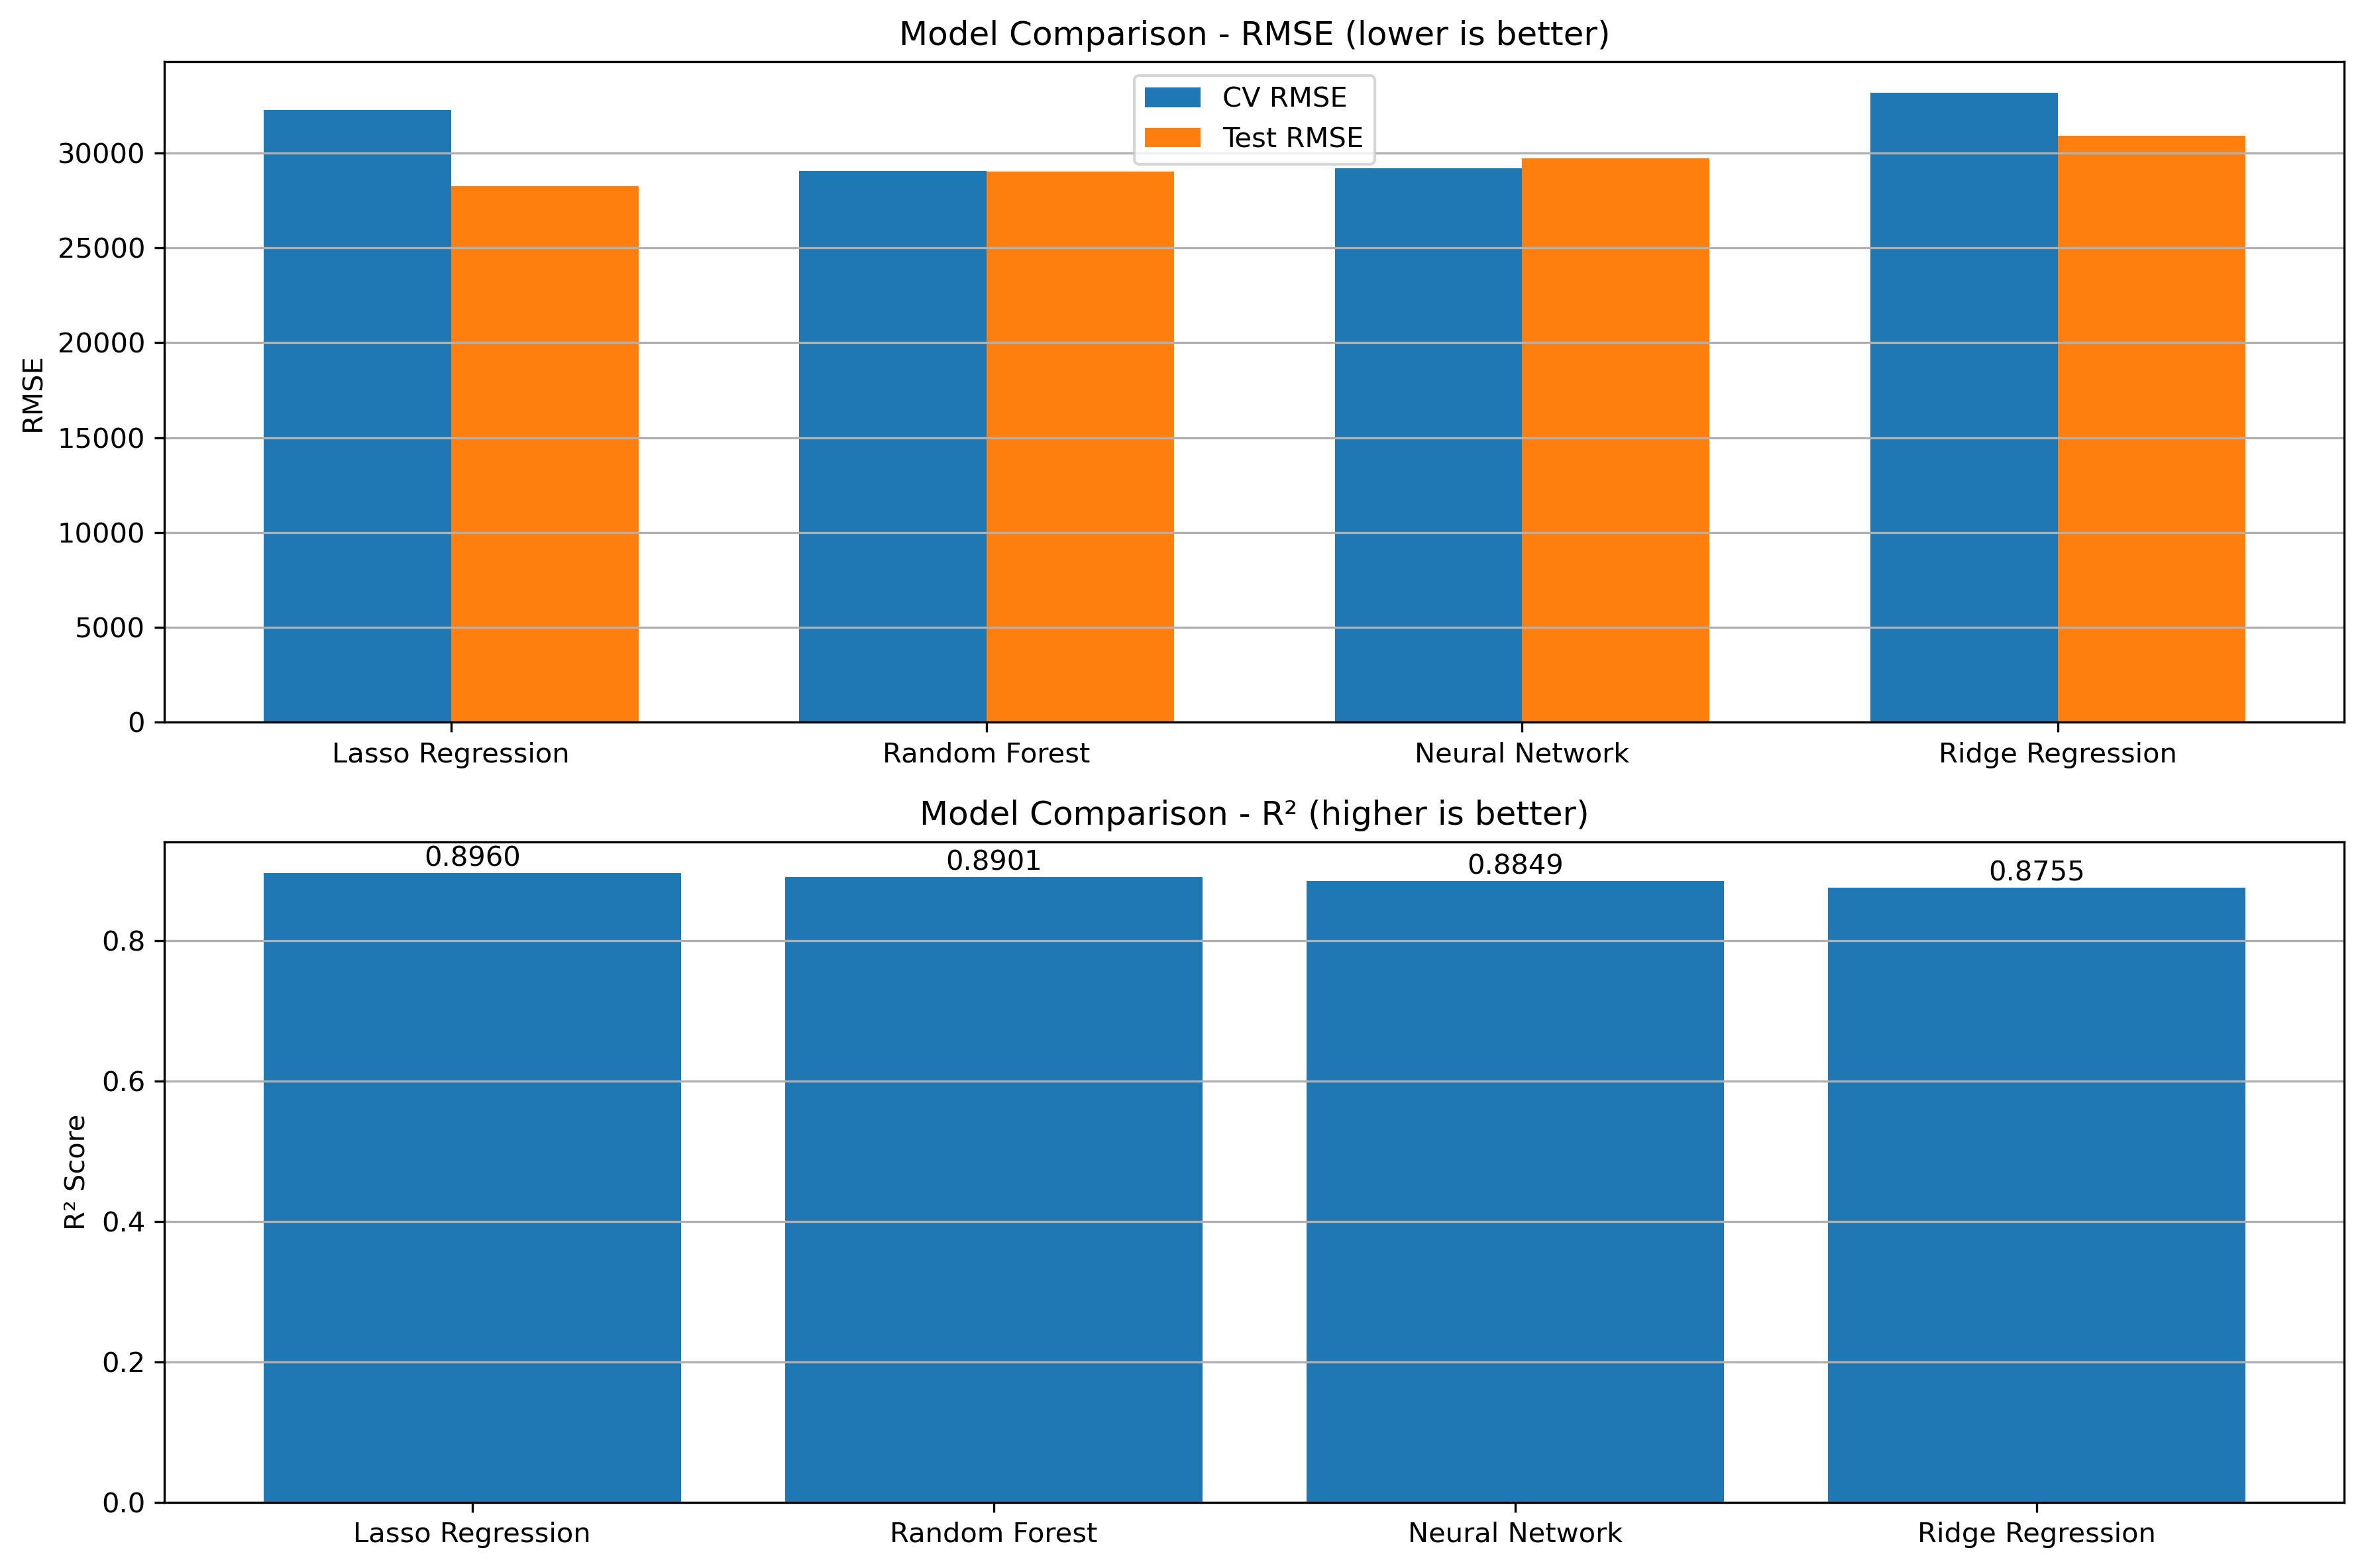
\includegraphics[width=1.0\textwidth]{figures/model_comparison.png}
    \caption{Performance Comparison Across Models}
    \label{fig:model_comparison}
\end{figure}

\subsection{Prediction Analysis}
\begin{figure}[H]
    \centering
    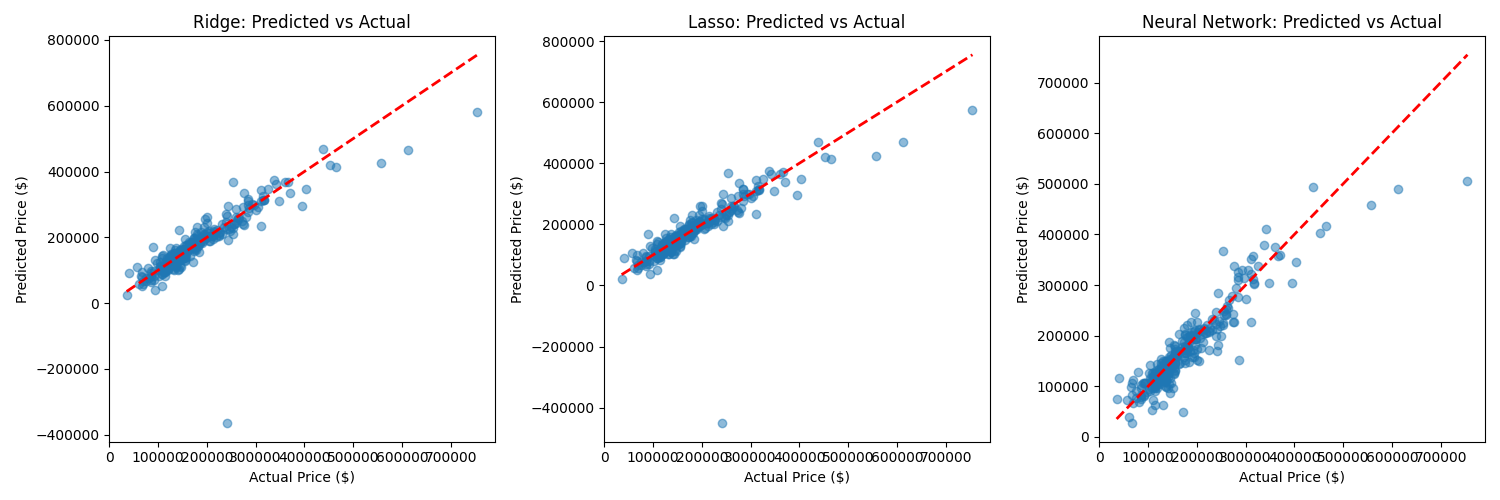
\includegraphics[width=1.0\textwidth]{figures/prediction_comparison.png}
    \caption{Prediction Comparison Between Models}
    \label{fig:prediction_comparison}
\end{figure}

Comparative analysis reveals:
\begin{itemize}
    \item Both Ridge and Lasso achieve similar optimal performance (RMSE ≈ 33,839)
    \item Linear models (Ridge and Lasso) provide good interpretability
    \item Neural network captures complex non-linear relationships
    \item Model ensemble potential for improved predictions
\end{itemize}

\section{Key Findings and Recommendations}
Based on the comprehensive modeling analysis:
\begin{itemize}
    \item Ridge Regression:
    \begin{itemize}
        \item Best for handling multicollinearity
        \item Provides stable feature importance estimates
        \item Achieves optimal performance at lambda ≈ 1048
    \end{itemize}
    \item Lasso Regression:
    \begin{itemize}
        \item Offers automatic feature selection
        \item Produces sparse solutions
        \item Shows similar optimal lambda value to Ridge
    \end{itemize}
    \item Neural Network:
    \begin{itemize}
        \item Captures complex non-linear relationships
        \item Shows potential for high accuracy
        \item Requires more data for optimal performance
    \end{itemize}
\end{itemize}

\section{Future Improvements}
Potential enhancements for model performance:
\begin{itemize}
    \item Ensemble methods combining multiple models
    \item Feature engineering based on domain knowledge
    \item Hyperparameter optimization through cross-validation
    \item Integration of temporal market trends
    \item Neighborhood-specific sub-models
\end{itemize}

\end{document} 